%%%%%%%%%%%%%%%%%%%%%%%%%%%%%%%%%%%%%%%%%%%%%%%%%%%%%%%%%%%%%%%%%%%%%%%%%%%%%
%% 03_arch_memory_concept.tex
%% Section: Memory Concept
%% Chapter: Architecture Concepts
%%
%% Describes the two-level cache hierarchy (I-Cache / D-Cache),
%% tag/data array organisation, replacement policy, the CPU-to-Cache
%% interface, the AXI4 bus between cache controllers and the Memory
%% Arbiter, and the read path to NOR Flash via QSPI.
%%
%% Status: v0.1 -- initial draft, subject to refinement.
%%
%% Integration in 00_rwurv64i_all.tex:
%%   \section{Memory Concept}
%%   \input{\TEXTarch 03_arch_history_tab07}
%%   \input{\TEXTarch 03_arch_memory_concept}
%%
%% Requires packages: tabularx, booktabs, tikz, float, xcolor, amsmath
%%%%%%%%%%%%%%%%%%%%%%%%%%%%%%%%%%%%%%%%%%%%%%%%%%%%%%%%%%%%%%%%%%%%%%%%%%%%%

%%%%%%%%%%%%%%%%%%%%%%%%%%%%%%%%%%%%%%%%%%%%%%%%%%%%%%%%%%%%%%%%%%%%%%%%%%%%%
\subsection{Overview}
%%%%%%%%%%%%%%%%%%%%%%%%%%%%%%%%%%%%%%%%%%%%%%%%%%%%%%%%%%%%%%%%%%%%%%%%%%%%%

The RWU-RV64I chip uses a Harvard-style split-cache architecture.
A dedicated \textbf{Instruction Cache (I-Cache)} serves the CPU fetch path,
and a dedicated \textbf{Data Cache (D-Cache)} serves the load/store path.
Both caches are 4-way set-associative with a fixed cache-line size of
32\,bytes.

The backing store for both caches is an off-chip \textbf{NOR Flash} memory
accessed through the on-chip QSPI controller.
NOR Flash is read-only from the cache's perspective; accordingly the D-Cache
operates as a \textbf{read-allocate, no-write-back} cache for the Flash
address region.
Cache data is held in two on-chip \textbf{SRAM macros} (X-Fab process),
one per cache.
A \textbf{Memory Arbiter} serialises simultaneous miss requests from the two
cache controllers onto the single AXI4 bus that leads to the QSPI controller.

Read-write data (stack, heap, \texttt{.data}, \texttt{.bss}) resides in a
dedicated on-chip \textbf{Scratchpad SRAM}.
The D-Cache controller decodes the physical address of every load/store: if
the address falls in the Flash region the request is served through the cache;
if it falls in the Scratchpad region the cache is bypassed and the Scratchpad
SRAM is accessed directly via a simple synchronous interface.
Because the scratchpad is uncacheable, dirty evictions from the D-Cache
can never occur; the dirty bit and the write-back FSM state are therefore
eliminated.

The on-chip bus between cache controllers and the Memory Arbiter uses a
subset of the \textbf{AMBA AXI4} protocol with burst support, replacing the
Wishbone B4 Classic interface used elsewhere in the design.
This allows a full 32-byte cache-line fill to complete in a single
four-beat burst transaction instead of eight independent single transfers.

\begin{table}[H]
\caption{Memory Hierarchy Summary}
\label{tab:asMemHierarchy}
\centering
\begin{tabularx}{\textwidth}{|l |l |l |l |X|}
  \hline
  Level & Block & Capacity & Technology & Latency (typical) \\
  \hline
  \hline
  L1-I & I-Cache    & 4\,KB (param.)  & On-chip SRAM macro  & 1 cycle (hit) \\
  \hline
  L1-D & D-Cache    & 4\,KB (param.)  & On-chip SRAM macro  & 1 cycle (hit) \\
  \hline
  --   & Scratchpad & TBD (param.)    & On-chip SRAM macro  & 1--2 cycles (direct) \\
  \hline
  Main & NOR Flash  & device-specific & Off-chip via QSPI   & \(\gg\)10 cycles (miss) \\
  \hline
\end{tabularx}
\end{table}

%%%%%%%%%%%%%%%%%%%%%%%%%%%%%%%%%%%%%%%%%%%%%%%%%%%%%%%%%%%%%%%%%%%%%%%%%%%%%
\subsection{System Memory Architecture}
%%%%%%%%%%%%%%%%%%%%%%%%%%%%%%%%%%%%%%%%%%%%%%%%%%%%%%%%%%%%%%%%%%%%%%%%%%%%%

Figure~\ref{fig:asMemArch01} shows the system-level block diagram of the
memory subsystem.

\begin{figure}[H]
\centering
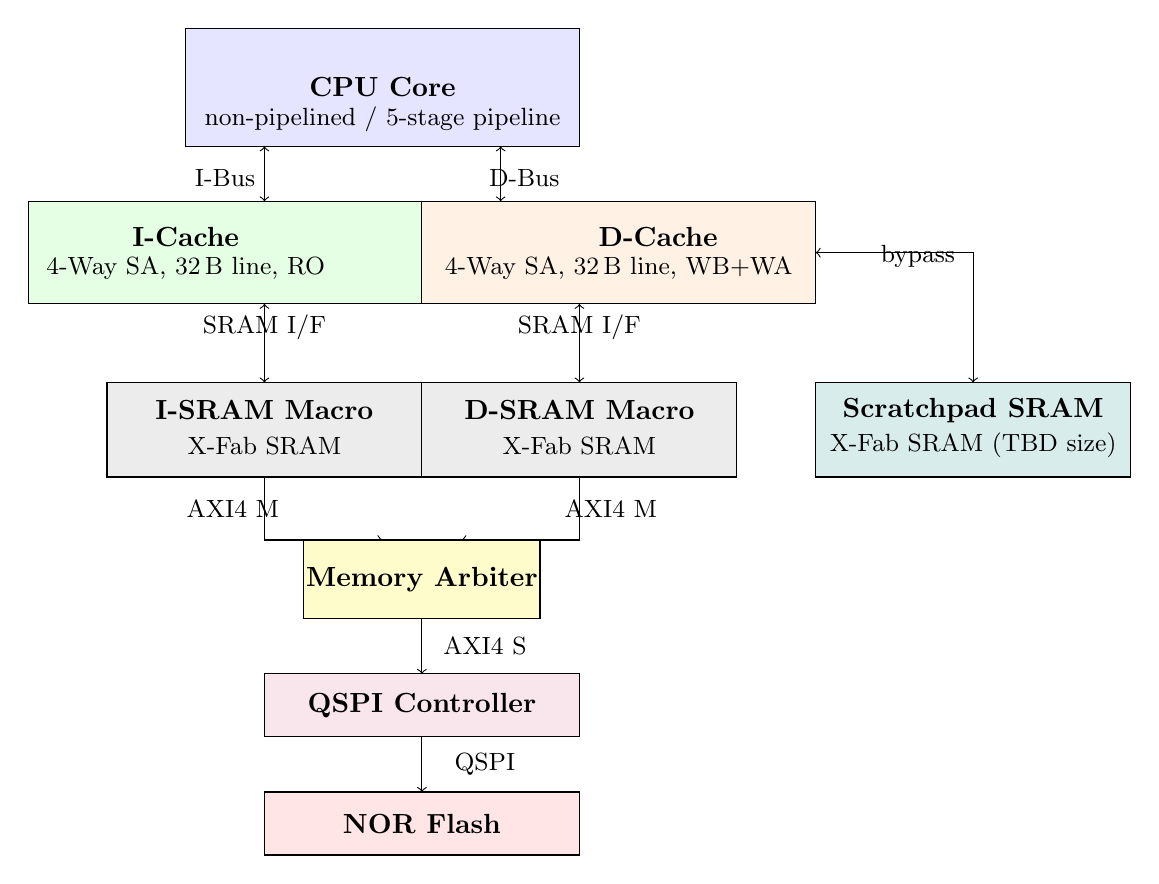
\begin{tikzpicture}[x=1cm, y=1cm]

  % CPU box
  \filldraw[fill=blue!10, draw=black] (3.5,10.5) rectangle (8.5,12);
  \node[align=center] at (6,11.25) {\textbf{CPU Core}};
  \node[align=center,font=\small] at (6,10.85) {non-pipelined / 5-stage pipeline};

  % Instruction Bus label
  \node[font=\small] at (4.0,10.1) {I-Bus};
  \draw[<->] (4.5,10.5) -- (4.5,9.8);

  % Data Bus label
  \node[font=\small] at (7.8,10.1) {D-Bus};
  \draw[<->] (7.5,10.5) -- (7.5,9.8);

  % I-Cache box
  \filldraw[fill=green!10, draw=black] (1.5,8.5) rectangle (6.5,9.8);
  \node[align=center] at (3.5,9.35) {\textbf{I-Cache}};
  \node[align=center,font=\small] at (3.5,8.95) {4-Way SA, 32\,B line, RO};

  % D-Cache box
  \filldraw[fill=orange!10, draw=black] (6.5,8.5) rectangle (11.5,9.8);
  \node[align=center] at (9.5,9.35) {\textbf{D-Cache}};
  \node[align=center,font=\small] at (9.0,8.95) {4-Way SA, 32\,B line, WB+WA};

  % I-SRAM label and arrow
  \node[font=\small] at (4.5,8.2) {SRAM I/F};
  \draw[<->] (4.5,8.5) -- (4.5,7.5);

  % D-SRAM label and arrow
  \node[font=\small] at (8.5,8.2) {SRAM I/F};
  \draw[<->] (8.5,8.5) -- (8.5,7.5);

  % I-SRAM Macro
  \filldraw[fill=gray!15, draw=black] (2.5,6.3) rectangle (6.5,7.5);
  \node[align=center] at (4.5,7.15) {\textbf{I-SRAM Macro}};
  \node[align=center,font=\small] at (4.5,6.7) {X-Fab SRAM};

  % D-SRAM Macro
  \filldraw[fill=gray!15, draw=black] (6.5,6.3) rectangle (10.5,7.5);
  \node[align=center] at (8.5,7.15) {\textbf{D-SRAM Macro}};
  \node[align=center,font=\small] at (8.5,6.7) {X-Fab SRAM};

  % Scratchpad SRAM Macro (bypass from D-Cache, right side)
  \filldraw[fill=teal!15, draw=black] (11.5,6.3) rectangle (15.5,7.5);
  \node[align=center] at (13.5,7.15) {\textbf{Scratchpad SRAM}};
  \node[align=center,font=\small] at (13.5,6.7) {X-Fab SRAM (TBD size)};

  % Bypass arrow D-Cache -> Scratchpad
  \node[font=\small] at (12.8,9.1) {bypass};
  \draw[<->] (11.5,9.15) -- (13.5,9.15) -- (13.5,7.5);

  % AXI4 arrows to arbiter
  \node[font=\small] at (4.1,5.9) {AXI4 M};
  \draw[->] (4.5,6.3) -- (4.5,5.5) -- (6.0,5.5);
  \node[font=\small] at (8.9,5.9) {AXI4 M};
  \draw[->] (8.5,6.3) -- (8.5,5.5) -- (7.0,5.5);

  % Memory Arbiter
  \filldraw[fill=yellow!20, draw=black] (5.0,4.5) rectangle (8.0,5.5);
  \node[align=center] at (6.5,5.0) {\textbf{Memory Arbiter}};

  % Arrow to QSPI
  \draw[->] (6.5,4.5) -- (6.5,3.8);
  \node[font=\small] at (7.3,4.15) {AXI4 S};

  % QSPI Controller
  \filldraw[fill=purple!10, draw=black] (4.5,3.0) rectangle (8.5,3.8);
  \node[align=center] at (6.5,3.4) {\textbf{QSPI Controller}};

  % Arrow to NOR Flash
  \draw[->] (6.5,3.0) -- (6.5,2.3);
  \node[font=\small] at (7.3,2.65) {QSPI};

  % NOR Flash
  \filldraw[fill=red!10, draw=black] (4.5,1.5) rectangle (8.5,2.3);
  \node[align=center] at (6.5,1.9) {\textbf{NOR Flash}};

\end{tikzpicture}
\caption{System Memory Architecture Block Diagram}
\label{fig:asMemArch01}
\end{figure}

%%%%%%%%%%%%%%%%%%%%%%%%%%%%%%%%%%%%%%%%%%%%%%%%%%%%%%%%%%%%%%%%%%%%%%%%%%%%%
\subsection{Cache Configuration Parameters}
%%%%%%%%%%%%%%%%%%%%%%%%%%%%%%%%%%%%%%%%%%%%%%%%%%%%%%%%%%%%%%%%%%%%%%%%%%%%%

Both caches share the same structural parameters, listed in
Table~\ref{tab:asCacheParams}.
Parameters marked \emph{fixed} are part of the cache-line protocol and
cannot be changed without redesigning the AXI4 burst transactions and the
SRAM macros.

\begin{table}[H]
\caption{Cache Configuration Parameters}
\label{tab:asCacheParams}
\centering
\begin{tabularx}{\textwidth}{|l |l |l |l |X|}
  \hline
  Parameter & Symbol & Default & Fixed? & Description \\
  \hline
  \hline
  Cache size          & \texttt{CACHE\_SIZE\_B} & 4096 & no  & Total capacity in bytes per cache \\
  \hline
  Associativity       & \texttt{WAYS}           & 4    & yes & Number of ways per set \\
  \hline
  Cache-line size     & \texttt{LINE\_BYTES}    & 32   & yes & Bytes per cache line \\
  \hline
  Number of sets      & \texttt{SETS}           & 32   & no  & Derived: \texttt{CACHE\_SIZE\_B / (WAYS * LINE\_BYTES)} \\
  \hline
  Physical addr width & \texttt{PA\_WIDTH}      & 32   & no  & Physical address bits \\
  \hline
  AXI4 data width     & \texttt{AXI\_DW}        & 64   & yes & AXI4 memory bus data width \\
  \hline
\end{tabularx}
\end{table}

%%%%%%%%%%%%%%%%%%%%%%%%%%%%%%%%%%%%%%%%%%%%%%%%%%%%%%%%%%%%%%%%%%%%%%%%%%%%%
\subsection{Physical Address Decomposition}
%%%%%%%%%%%%%%%%%%%%%%%%%%%%%%%%%%%%%%%%%%%%%%%%%%%%%%%%%%%%%%%%%%%%%%%%%%%%%

With the default parameters (4\,KB cache, 4-way, 32\,B line, 32-bit
physical address), a physical address is divided as shown in
Figure~\ref{fig:asAddrDecomp} and Table~\ref{tab:asAddrFields}.

\begin{figure}[H]
\centering
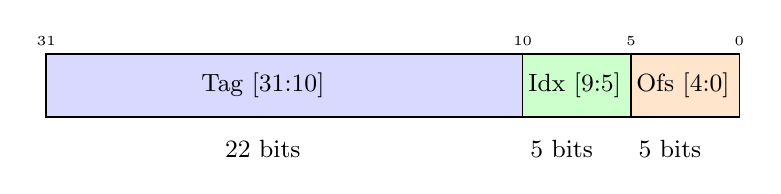
\begin{tikzpicture}[x=0.55cm, y=0.8cm]
  % full address bar
  \draw[thick] (0,0) rectangle (16,1);
  % tag field [31:10]
  \filldraw[fill=blue!15, draw=black] (0,0) rectangle (11,1);
  \node at (5,0.5) {\small Tag [31:10]};
  \node[font=\tiny] at (11,1.2) {10};
  \node[font=\tiny] at (0,1.2) {31};
  % index field [9:5]
  \filldraw[fill=green!20, draw=black] (11,0) rectangle (13.5,1);
  \node at (12.2,0.5) {\small Idx [9:5]};
  \node[font=\tiny] at (13.5,1.2) {5};
  % offset field [4:0]
  \filldraw[fill=orange!20, draw=black] (13.5,0) rectangle (16,1);
  \node at (14.7,0.5) {\small Ofs [4:0]};
  \node[font=\tiny] at (16,1.2) {0};
  % bit annotations
  \node[font=\small] at (5,-0.5) {22 bits};
  \node[font=\small] at (11.9,-0.5) {5 bits};
  \node[font=\small] at (14.4,-0.5) {5 bits};
\end{tikzpicture}
\caption{Physical Address Decomposition (32-bit PA, 4\,KB cache, 32\,B line)}
\label{fig:asAddrDecomp}
\end{figure}

\begin{table}[H]
\caption{Physical Address Fields}
\label{tab:asAddrFields}
\centering
\begin{tabularx}{\textwidth}{|l |l |l |X|}
  \hline
  Field & Bits & Width & Description \\
  \hline
  \hline
  \texttt{tag}    & [31:10] & 22 & Compared against stored tag to determine hit/miss \\
  \hline
  \texttt{index}  & [9:5]   & 5  & Selects one of 32 sets \\
  \hline
  \texttt{offset} & [4:0]   & 5  & Byte offset within the 32-byte cache line \\
  \hline
  \texttt{word}   & [4:3]   & 2  & Selects one of four 64-bit words within the line \\
  \hline
  \texttt{instr}  & [4:2]   & 3  & Selects one of eight 32-bit instructions (I-Cache only) \\
  \hline
  \texttt{byte}   & [2:0]   & 3  & Byte offset within a 64-bit word (D-Cache sub-word) \\
  \hline
\end{tabularx}
\end{table}

The general formula for derived address parameters is:
\[
  \text{OFFSET\_BITS} = \log_2(\texttt{LINE\_BYTES}) = 5
\]
\[
  \text{INDEX\_BITS}  = \log_2(\texttt{SETS}) = \log_2\!\left(\frac{\texttt{CACHE\_SIZE\_B}}{\texttt{WAYS} \times \texttt{LINE\_BYTES}}\right) = 5
\]
\[
  \text{TAG\_BITS} = \texttt{PA\_WIDTH} - \text{INDEX\_BITS} - \text{OFFSET\_BITS} = 32 - 5 - 5 = 22
\]

%%%%%%%%%%%%%%%%%%%%%%%%%%%%%%%%%%%%%%%%%%%%%%%%%%%%%%%%%%%%%%%%%%%%%%%%%%%%%
\subsection{Cache Tag and Metadata Arrays}
%%%%%%%%%%%%%%%%%%%%%%%%%%%%%%%%%%%%%%%%%%%%%%%%%%%%%%%%%%%%%%%%%%%%%%%%%%%%%

Each set contains per-way metadata (valid, tag, and for D-Cache: dirty bit)
plus shared set-level pseudo-LRU bits.

\subsubsection{I-Cache Metadata Layout}

The I-Cache is read-only; no dirty bit is required.

\begin{table}[H]
\caption{I-Cache -- Metadata Bits per Set}
\label{tab:asICacheTag}
\centering
\begin{tabularx}{\textwidth}{|l |l |l |X|}
  \hline
  Field & Bits & Width & Description \\
  \hline
  \hline
  \multicolumn{4}{|l|}{Per way (repeated 4$\times$):} \\
  \hline
  \texttt{valid[w]}  & 1 per way  & 1  & Line present in cache; cleared on reset or flush \\
  \hline
  \texttt{tag[w]}    & 22 per way & 22 & Upper address bits stored at fill time \\
  \hline
  \multicolumn{4}{|l|}{Per set (shared):} \\
  \hline
  \texttt{plru[2:0]} & 3 per set  & 3  & Pseudo-LRU replacement state (see Section~\ref{subsec:plru}) \\
  \hline
  \multicolumn{4}{|l|}{Total per set:} \\
  \hline
  (sum) & -- & 95 & $4 \times (1+22) + 3 = 95$\,bits; rounded to 96 for SRAM alignment \\
  \hline
\end{tabularx}
\end{table}

\subsubsection{D-Cache Metadata Layout}

The D-Cache is read-allocate with no write-back; no dirty bit is required
(identical structure to the I-Cache metadata).

\begin{table}[H]
\caption{D-Cache -- Metadata Bits per Set}
\label{tab:asDCacheTag}
\centering
\begin{tabularx}{\textwidth}{|l |l |l |X|}
  \hline
  Field & Bits & Width & Description \\
  \hline
  \hline
  \multicolumn{4}{|l|}{Per way (repeated 4$\times$):} \\
  \hline
  \texttt{valid[w]}  & 1 per way  & 1  & Line present in cache; cleared on reset or flush \\
  \hline
  \texttt{tag[w]}    & 22 per way & 22 & Tag stored at fill time \\
  \hline
  \multicolumn{4}{|l|}{Per set (shared):} \\
  \hline
  \texttt{plru[2:0]} & 3 per set  & 3  & Pseudo-LRU replacement state (see Section~\ref{subsec:plru}) \\
  \hline
  \multicolumn{4}{|l|}{Total per set:} \\
  \hline
  (sum) & -- & 95 & $4 \times (1+22) + 3 = 95$\,bits; rounded to 96 for SRAM alignment \\
  \hline
\end{tabularx}
\end{table}

\subsubsection{Pseudo-LRU Replacement Policy}
\label{subsec:plru}

A 3-bit pseudo-LRU (PLRU) binary tree approximates LRU replacement for
4~ways without the overhead of true LRU.
The tree is shown in Figure~\ref{fig:asPlru} and the bit semantics are
defined in Table~\ref{tab:asPlruBits}.

\begin{figure}[H]
\centering
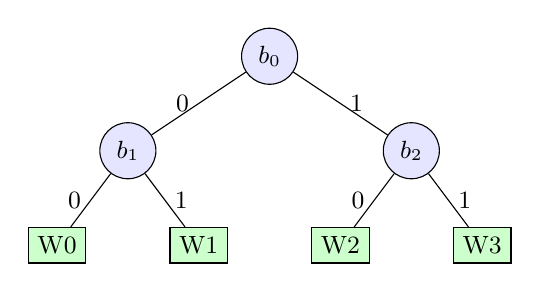
\begin{tikzpicture}[x=1.2cm, y=1.2cm]
  \node[draw, circle, fill=blue!10] (b0) at (3,3) {\small $b_0$};
  \node[draw, circle, fill=blue!10] (b1) at (1.5,2) {\small $b_1$};
  \node[draw, circle, fill=blue!10] (b2) at (4.5,2) {\small $b_2$};
  \node[draw, fill=green!20] (w0) at (0.75,1) {\small W0};
  \node[draw, fill=green!20] (w1) at (2.25,1) {\small W1};
  \node[draw, fill=green!20] (w2) at (3.75,1) {\small W2};
  \node[draw, fill=green!20] (w3) at (5.25,1) {\small W3};
  \draw (b0) -- node[left,font=\small]{0} (b1);
  \draw (b0) -- node[right,font=\small]{1} (b2);
  \draw (b1) -- node[left,font=\small]{0} (w0);
  \draw (b1) -- node[right,font=\small]{1} (w1);
  \draw (b2) -- node[left,font=\small]{0} (w2);
  \draw (b2) -- node[right,font=\small]{1} (w3);
\end{tikzpicture}
\caption{Pseudo-LRU Binary Tree for 4 Ways}
\label{fig:asPlru}
\end{figure}

\begin{table}[H]
\caption{PLRU Bit Semantics}
\label{tab:asPlruBits}
\centering
\begin{tabularx}{\textwidth}{|l |X |X|}
  \hline
  Bit & Meaning (bit=0) & Meaning (bit=1) \\
  \hline
  \hline
  $b_0$ & Left pair (W0, W1) is LRU; victim from left half & Right pair (W2, W3) is LRU; victim from right half \\
  \hline
  $b_1$ & W1 is LRU within left pair; evict W1 & W0 is LRU within left pair; evict W0 \\
  \hline
  $b_2$ & W3 is LRU within right pair; evict W3 & W2 is LRU within right pair; evict W2 \\
  \hline
\end{tabularx}
\end{table}

Victim selection and PLRU update rules are defined in Table~\ref{tab:asPlruUpdate}.

\begin{table}[H]
\caption{PLRU Victim Selection and Update on Cache Access}
\label{tab:asPlruUpdate}
\centering
\begin{tabularx}{\textwidth}{|l |l |X|}
  \hline
  Accessed Way & Victim (for miss/eviction) & PLRU bits updated \\
  \hline
  \hline
  W0 & $b_0$=0: ($b_1$=0~$\Rightarrow$ W1), ($b_1$=1~$\Rightarrow$ W0) & $b_0 \leftarrow 1$,\; $b_1 \leftarrow 1$ \\
  \hline
  W1 & same left half & $b_0 \leftarrow 1$,\; $b_1 \leftarrow 0$ \\
  \hline
  W2 & $b_0$=1: ($b_2$=0~$\Rightarrow$ W3), ($b_2$=1~$\Rightarrow$ W2) & $b_0 \leftarrow 0$,\; $b_2 \leftarrow 1$ \\
  \hline
  W3 & same right half & $b_0 \leftarrow 0$,\; $b_2 \leftarrow 0$ \\
  \hline
\end{tabularx}
\end{table}

The PLRU state is stored in a small register array (32 sets $\times$ 3 bits = 96 bits).
It is reset to all-zero on power-on reset.

%%%%%%%%%%%%%%%%%%%%%%%%%%%%%%%%%%%%%%%%%%%%%%%%%%%%%%%%%%%%%%%%%%%%%%%%%%%%%
\subsection{SRAM Macro Organisation}
%%%%%%%%%%%%%%%%%%%%%%%%%%%%%%%%%%%%%%%%%%%%%%%%%%%%%%%%%%%%%%%%%%%%%%%%%%%%%

The memory subsystem uses five X-Fab XO035 SPRAM macros in total
(see Section~\ref{subsec:sramSelection} for the selected instances).
All macros operate as single-port synchronous SRAMs at 3.3\,V.

\begin{table}[H]
\caption{SRAM Macro Logical Requirements}
\label{tab:asSramMacros}
\centering
\begin{tabularx}{\textwidth}{|l |l |l |l |X|}
  \hline
  Macro & Width & Depth & Size & Notes \\
  \hline
  \hline
  Tag SRAM (I)  & 96\,bit  & 32   & 384\,B   & valid + tag for 4 ways + 3 PLRU bits; rounded from 95 \\
  \hline
  Tag SRAM (D)  & 96\,bit  & 32   & 384\,B   & same structure as I-Cache (no dirty bit); rounded from 95 \\
  \hline
  Data SRAM (I) & 256\,bit & 128  & 4\,KB    & 32 sets $\times$ 4 ways $\times$ 32\,B; addressed as \texttt{\{index,way\}} \\
  \hline
  Data SRAM (D) & 256\,bit & 128  & 4\,KB    & same organisation as I-Cache data SRAM \\
  \hline
  Scratchpad    & 64\,bit  & \texttt{SP\_DEPTH} & \texttt{SP\_SIZE\_B} &
    Default: \texttt{SP\_DEPTH=1024} $\Rightarrow$ 8\,KB;
    addressed by \texttt{dc\_addr\_i[12:3]} \\
  \hline
\end{tabularx}
\end{table}

The data SRAM is addressed by the concatenation \texttt{\{index[4:0], way[1:0]\}}
giving a 7-bit address (128 entries).
All 256 bits of one cache line are read or written in a single SRAM cycle.

During a cache-line fill, the cache controller writes the four 64-bit AXI4
beat words into the data SRAM on four consecutive cycles using a word-level
write enable, while the full line address (\texttt{index} $\parallel$
\texttt{fill\_way}) is held constant.

The Scratchpad SRAM is accessed with a 64-bit data bus and an 8-bit byte
enable (\texttt{dc\_wstrb\_i}), matching the D-Cache data bus width.
Its address is derived directly from \texttt{dc\_addr\_i[12:3]} (for the
default 8\,KB instance).

%%%%%%%%%%%%%%%%%%%%%%%%%%%%%%%%%%%%%%%%%%%%%%%%%%%%%%%%%%%%%%%%%%%%%%%%%%%%%
\subsection{SRAM Macro Selection -- XO035 SPRAM}
\label{subsec:sramSelection}
%%%%%%%%%%%%%%%%%%%%%%%%%%%%%%%%%%%%%%%%%%%%%%%%%%%%%%%%%%%%%%%%%%%%%%%%%%%%%

\subsubsection{Library and Process}

All SRAM macros are generated with the X-Fab \textbf{XO035}
(350\,nm Modular Sensor Technology Platform)
\textbf{SPRAM} (Single-Port RAM) compiler at the nominal supply of
3.3\,V (2.2\,V low-voltage option not used).
Key library properties relevant to this design:

\begin{itemize}
  \item Zero static DC power consumption (only intrinsic leakage).
  \item Separate input and output data buses (no bus contention during
    read-modify-write).
  \item Byte-level write enable supported (required for sub-word stores
    to the Scratchpad SRAM).
  \item Wide range of instance sizes; the compiler generates macros for
    the exact width$\times$depth parameters listed in
    Table~\ref{tab:asSramInstances}.
  \item Optional BIST block: \textbf{not instantiated} in the first
    tapeout; test coverage via scan chain is sufficient.
\end{itemize}

\subsubsection{Selected Instances}

Table~\ref{tab:asSramInstances} lists the five SPRAM instances to be
generated from the XO035 compiler.
Macro names follow the compiler naming convention and are to be confirmed
against the current catalogue release.

\begin{table}[H]
\caption{XO035 SPRAM Instances}
\label{tab:asSramInstances}
\centering
\begin{tabularx}{\textwidth}{|l |l |l |l |l |X|}
  \hline
  Instance & Width & Depth & Size & Macro name & Usage \\
  \hline
  \hline
  I-Tag  & 96\,bit  & 32   & 384\,B & \texttt{SPRAM\_96x32}   & I-Cache tag + valid + PLRU \\
  \hline
  D-Tag  & 96\,bit  & 32   & 384\,B & \texttt{SPRAM\_96x32}   & D-Cache tag + valid + PLRU \\
  \hline
  I-Data & 256\,bit & 128  & 4\,KB  & \texttt{SPRAM\_256x128} & I-Cache data array \\
  \hline
  D-Data & 256\,bit & 128  & 4\,KB  & \texttt{SPRAM\_256x128} & D-Cache data array \\
  \hline
  SP     & 64\,bit  & 1024 & 8\,KB  & \texttt{SPRAM\_64x1024} & Scratchpad (stack/heap/.data/.bss) \\
  \hline
\end{tabularx}
\end{table}

\textbf{Notes on macro names:}
The names \texttt{SPRAM\_\{W\}x\{D\}} are placeholders using the pattern
$\langle$width$\rangle$x$\langle$depth$\rangle$.
The actual names generated by the XO035 SPRAM compiler must be verified
against the compiler catalogue and substituted in the netlist and
floorplan before tapeout.
I-Tag and D-Tag use the \emph{same} compiled macro; two instances are
placed.
I-Data and D-Data likewise share one compiled macro with two instances.

\subsubsection{SRAM Port Mapping}

Table~\ref{tab:asSramPorts} maps the logical cache-controller signals
to the standard XO035 SPRAM port names.

\begin{table}[H]
\caption{XO035 SPRAM Port Mapping}
\label{tab:asSramPorts}
\centering
\begin{tabularx}{\textwidth}{|l |l |X|}
  \hline
  SPRAM port & Direction & Connected to \\
  \hline
  \hline
  \texttt{CLK}  & in  & System clock \texttt{clk\_i} \\
  \hline
  \texttt{CEN}  & in  & Chip enable, active-low; asserted when cache controller
                        drives a valid address \\
  \hline
  \texttt{WEN}  & in  & Write enable, active-low; low for write, high for read \\
  \hline
  \texttt{BWEN} & in  & Bit-write enable, active-low; all-zero = write all bits
                        (tag/data SRAMs); \texttt{\textasciitilde dc\_wstrb\_i}
                        expanded to bit-level (Scratchpad only) \\
  \hline
  \texttt{A}    & in  & Address bus; see Table~\ref{tab:asSramMacros} for width \\
  \hline
  \texttt{D}    & in  & Write data \\
  \hline
  \texttt{Q}    & out & Read data; valid one cycle after \texttt{CEN} low on a read \\
  \hline
\end{tabularx}
\end{table}

\subsubsection{Timing Parameters}

Table~\ref{tab:asSramTiming} lists the timing parameters to be extracted
from the XO035 SPRAM compiler output for the worst-case process corner
(SS -- slow NMOS, slow PMOS), maximum temperature (125\,\textdegree C),
and minimum supply voltage (3.0\,V for 3.3\,V nominal).

\begin{table}[H]
\caption{XO035 SPRAM Timing Parameters (worst-case SS/125\,\textdegree C/3.0\,V)}
\label{tab:asSramTiming}
\centering
\begin{tabularx}{\textwidth}{|l |l |l |X|}
  \hline
  Parameter & Symbol & Value & Description \\
  \hline
  \hline
  Clock period (min.) & $t_\text{cyc}$ & TBD\,ns & Minimum clock period for correct operation \\
  \hline
  Access time         & $t_\text{aa}$  & TBD\,ns & Address to \texttt{Q} valid; determines read latency \\
  \hline
  Setup time (data)   & $t_\text{ds}$  & TBD\,ns & \texttt{D} / \texttt{BWEN} setup before rising \texttt{CLK} \\
  \hline
  Hold time (data)    & $t_\text{dh}$  & TBD\,ns & \texttt{D} / \texttt{BWEN} hold after rising \texttt{CLK} \\
  \hline
  Setup time (addr.)  & $t_\text{as}$  & TBD\,ns & \texttt{A} / \texttt{CEN} / \texttt{WEN} setup before rising \texttt{CLK} \\
  \hline
  Hold time (addr.)   & $t_\text{ah}$  & TBD\,ns & \texttt{A} / \texttt{CEN} / \texttt{WEN} hold after rising \texttt{CLK} \\
  \hline
\end{tabularx}
\end{table}

The system clock frequency must satisfy:
\[
  f_\text{clk} \leq \frac{1}{t_\text{cyc,\,worst}}
\]
All cache hit paths (tag compare + data SRAM read) must close timing
within a single clock cycle at the selected frequency.
Static Timing Analysis (STA) with the compiler-supplied Liberty
(\texttt{.lib}) file is required before tapeout.

\textbf{Action (MEM-02):} Run the XO035 SPRAM compiler for all five
instances listed in Table~\ref{tab:asSramInstances} and fill in the
timing values in Table~\ref{tab:asSramTiming}.
Verify that the maximum target frequency is achievable at the SS/125\,\textdegree C/3.0\,V corner.

%%%%%%%%%%%%%%%%%%%%%%%%%%%%%%%%%%%%%%%%%%%%%%%%%%%%%%%%%%%%%%%%%%%%%%%%%%%%%
\subsection{Instruction Cache (I-Cache)}
%%%%%%%%%%%%%%%%%%%%%%%%%%%%%%%%%%%%%%%%%%%%%%%%%%%%%%%%%%%%%%%%%%%%%%%%%%%%%

\subsubsection{Functional Description}

The I-Cache is a read-only, 4-way set-associative cache that serves the
CPU instruction fetch stage.
It has no write path to the backing NOR Flash, and no dirty bit.

On every fetch request the cache controller:
\begin{enumerate}
  \item Reads the tag SRAM at address \texttt{index}.
  \item Compares the four stored tags with the request tag in parallel.
  \item Checks the corresponding valid bits.
  \item On a hit: reads the data SRAM at \texttt{\{index, hit\_way\}},
    selects the 32-bit instruction word using \texttt{offset[4:2]},
    and returns it to the CPU in the same cycle.
  \item On a miss: stalls the CPU, issues an AXI4 read burst to the
    Memory Arbiter, fills the selected SRAM line, updates the tag SRAM and
    PLRU state, then un-stalls the CPU.
\end{enumerate}

\subsubsection{Cache Hit Path}

The hit path is combinatorial: tag comparison, data SRAM read, and
instruction word selection complete within one clock cycle.
The CPU pipeline sees a zero-cycle miss overhead when the cache hits.

\subsubsection{Cache Miss Handling}

On a miss the I-Cache controller:
\begin{itemize}
  \item Uses the PLRU state to select the victim way.
  \item Asserts the \texttt{stall} signal to the CPU.
  \item Issues an AXI4 INCR burst of 4 beats (4 $\times$ 64\,bit = 32\,B)
    aligned to the cache-line boundary (\texttt{addr[63:5] \& 5'b0}).
  \item Writes the four beats sequentially into the data SRAM.
  \item Updates the tag and valid bit for the filled way.
  \item Updates the PLRU bits.
  \item De-asserts \texttt{stall} on the cycle the last beat arrives.
\end{itemize}

\subsubsection{I-Cache State Machine}
\label{subsec:icacheFsm}

\begin{table}[H]
\caption{I-Cache Controller States}
\label{tab:asICacheFsm}
\centering
\begin{tabularx}{\textwidth}{|l |X |}
  \hline
  State & Description \\
  \hline
  \hline
  \texttt{IDLE}      & Waiting for a fetch request or flush signal from the CPU \\
  \hline
  \texttt{LOOKUP}    & Tag comparison active; result available next cycle \\
  \hline
  \texttt{MISS}      & AXI4 AR channel: sending read address burst to arbiter \\
  \hline
  \texttt{FILL}      & Receiving 4 AXI4 R-channel beats; writing data SRAM \\
  \hline
  \texttt{RESPOND}   & First word of filled line presented to CPU; stall de-asserted \\
  \hline
  \texttt{ERR}       & AXI4 RRESP $\neq$ OKAY detected during FILL: valid bit not
                       set; \texttt{ic\_err\_o} pulsed high for one cycle;
                       return to IDLE \\
  \hline
  \texttt{FLUSH}     & Invalidation: iterates set counter 0\ldots31; writes
                       \texttt{valid=0}, \texttt{plru=0} to tag SRAM each cycle;
                       asserts \texttt{ic\_flush\_done\_o} after 32 cycles \\
  \hline
\end{tabularx}
\end{table}

%%%%%%%%%%%%%%%%%%%%%%%%%%%%%%%%%%%%%%%%%%%%%%%%%%%%%%%%%%%%%%%%%%%%%%%%%%%%%
\subsection{Data Cache (D-Cache)}
%%%%%%%%%%%%%%%%%%%%%%%%%%%%%%%%%%%%%%%%%%%%%%%%%%%%%%%%%%%%%%%%%%%%%%%%%%%%%

\subsubsection{Functional Description}

The D-Cache is a \textbf{read-allocate} 4-way set-associative cache that
serves the CPU load/store stage.
Sub-word accesses (byte, halfword, word, doubleword) are supported.

The D-Cache controller decodes the physical address of every CPU load/store
and dispatches to one of two paths:

\begin{itemize}
  \item \textbf{Flash region (cacheable, read-only):} the request goes
    through the tag-lookup / fill pipeline described below.
    Stores to the Flash region are not supported; the cache controller
    asserts \texttt{dc\_err\_o} and raises a Load Access Fault (see Section~\ref{subsec:axi4Error}).
  \item \textbf{Scratchpad region (uncacheable, read-write):} the cache is
    bypassed entirely.
    The controller drives the Scratchpad SRAM interface directly with the
    physical address, write data, byte enables, and read/write strobe, and
    returns the read data to the CPU after one SRAM cycle.
\end{itemize}

On a load from the Flash region the cache controller:
\begin{enumerate}
  \item Reads the tag SRAM at address \texttt{index}.
  \item Compares the four stored tags with the request tag in parallel.
  \item Checks the corresponding valid bits.
  \item On a read hit: reads the data SRAM, extracts the addressed word or
    sub-word, and returns it to the CPU in the same cycle.
  \item On a miss: stalls the CPU, issues an AXI4 read burst to the Memory
    Arbiter, fills the selected SRAM line, updates tag and valid bit,
    updates the PLRU state, then un-stalls the CPU.
\end{enumerate}

\subsubsection{Address Region Policy and Absence of Write-Back}

Because the Flash backing store is read-only and the Scratchpad is
uncacheable, \textbf{the dirty bit is never set} and no cache line is ever
marked for write-back.
As a direct consequence:

\begin{itemize}
  \item The D-Cache metadata does \textbf{not} contain a dirty bit
    (contrast with Table~\ref{tab:asDCacheTag}, which is superseded:
    the dirty field is removed; per-way metadata reduces from
    $(1+1+22)=24$ to $(1+22)=23$ bits).
  \item The \texttt{WRITEBACK} FSM state and the full AXI4 write path
    (AW, W, B channels) are \textbf{eliminated} from the D-Cache
    controller.
    The D-Cache requires only the AXI4 read channels (AR, R).
  \item Write-allocate is \textbf{not applicable}: stores go to the
    Scratchpad directly; there is no ``write miss'' into the cache.
\end{itemize}

This simplification resolves open item MEM-01 and reduces D-Cache
controller complexity significantly.

\subsubsection{Scratchpad SRAM -- Software Segment Mapping}
\label{subsubsec:scratchpadSegments}

The Scratchpad SRAM serves as the sole read-write memory of the system.
It holds all program data that must be writable at run time.
Table~\ref{tab:asScratchpadSegments} lists the standard linker segments
assigned to the Scratchpad region.

\begin{table}[H]
\caption{Software Segments in Scratchpad SRAM}
\label{tab:asScratchpadSegments}
\centering
\begin{tabularx}{\textwidth}{|l |l |X|}
  \hline
  Segment & Access & Content and lifecycle \\
  \hline
  \hline
  \texttt{.data} & R/W & Initialised global and static variables.
    Values are copied from NOR Flash to Scratchpad by the start-up
    routine (\texttt{\_start} / \texttt{crt0}) before \texttt{main()}
    is entered.
    Subsequent reads and writes go directly to Scratchpad. \\
  \hline
  \texttt{.bss}  & R/W & Uninitialised (zero-initialised) global and
    static variables.
    The start-up routine zeroes this region in Scratchpad before
    \texttt{main()} is entered; no NOR Flash copy is required. \\
  \hline
  Heap           & R/W & Dynamic memory managed by \texttt{malloc}/\texttt{free}
    (or equivalent).
    Grows upward from the end of \texttt{.bss} toward the stack.
    Access pattern is unpredictable (random reads and writes), making
    caching impractical. \\
  \hline
  Stack          & R/W & Automatic variables, function call frames,
    and saved registers.
    Grows downward from the top of the Scratchpad region.
    Access is highly regular (push/pop, mostly 8-byte aligned) but
    write-intensive; caching would require frequent dirty evictions. \\
  \hline
\end{tabularx}
\end{table}

\paragraph{Why these segments cannot reside in NOR Flash.}
NOR Flash is a read-only medium from the system's perspective: the QSPI
controller provides a cache-miss-driven read path only; there is no byte-
or word-level write path to Flash.
Even if write commands were issued via the QSPI configuration interface,
Flash write latency is in the millisecond range and requires sector erase
before re-programming -- wholly unsuitable for stack or heap access.

\paragraph{Linker script responsibility.}
The linker script must place \texttt{.data}, \texttt{.bss}, heap, and
stack inside the Scratchpad address window
(\texttt{SP\_BASE}\ldots\texttt{SP\_BASE + SP\_SIZE - 1}).
Code (\texttt{.text}) and read-only data (\texttt{.rodata}) remain in
the NOR Flash address window and are served through the cache.
The start-up routine copies \texttt{.data} from Flash to Scratchpad using
the D-Cache bypass path (Scratchpad addresses); the Flash source copy is
accessed through the D-Cache (Flash addresses).

\subsubsection{D-Cache State Machine}
\label{subsec:dcacheFsm}

\begin{table}[H]
\caption{D-Cache Controller States}
\label{tab:asDCacheFsm}
\centering
\begin{tabularx}{\textwidth}{|l |X |}
  \hline
  State & Description \\
  \hline
  \hline
  \texttt{IDLE}       & Waiting for a load/store request or flush signal from the CPU \\
  \hline
  \texttt{DECODE}     & Physical address decoded; dispatch to CACHE path (Flash region)
                        or BYPASS path (Scratchpad region) \\
  \hline
  \texttt{LOOKUP}     & Flash region: tag comparison active; result available next cycle \\
  \hline
  \texttt{FILL}       & Flash region: issuing AXI4 AR burst; receiving and writing
                        4 beats to data SRAM \\
  \hline
  \texttt{RESPOND}    & Flash region: read data presented to CPU; stall de-asserted \\
  \hline
  \texttt{BYPASS}     & Scratchpad region: driving Scratchpad SRAM interface directly;
                        read data or write acknowledgement returned to CPU after 1 cycle \\
  \hline
  \texttt{ERR}        & AXI4 RRESP $\neq$ OKAY detected during FILL: valid bit not
                        set; \texttt{dc\_err\_o} pulsed high for one cycle;
                        return to IDLE \\
  \hline
  \texttt{FLUSH}      & Invalidation: iterates set counter 0\ldots31; writes
                        \texttt{valid=0}, \texttt{plru=0} to tag SRAM each cycle;
                        asserts \texttt{dc\_flush\_done\_o} after 32 cycles \\
  \hline
\end{tabularx}
\end{table}

\textbf{Note:} The \texttt{WRITEBACK} and \texttt{WRITE\_HIT} states present
in earlier revisions of this document are removed.
Neither state can be reached: no dirty lines exist (Flash is read-only) and
stores bypass the cache via the \texttt{BYPASS} state.

%%%%%%%%%%%%%%%%%%%%%%%%%%%%%%%%%%%%%%%%%%%%%%%%%%%%%%%%%%%%%%%%%%%%%%%%%%%%%
\subsection{CPU-to-Cache Interface}
%%%%%%%%%%%%%%%%%%%%%%%%%%%%%%%%%%%%%%%%%%%%%%%%%%%%%%%%%%%%%%%%%%%%%%%%%%%%%

The interface between the CPU core and each cache uses a simple
valid/ready + stall handshake.
It is not based on Wishbone or AXI4: those protocols are reserved for
the off-chip memory path.

\subsubsection{Instruction Bus (CPU -- I-Cache)}
\label{subsec:iBusIf}

The Instruction Bus carries instruction fetch requests from the IF stage
to the I-Cache.

\begin{table}[H]
\caption{Instruction Bus Interface (\texttt{as\_icache\_if})}
\label{tab:asIBusIO}
\centering
\begin{tabularx}{\textwidth}{|l |l |l |X|}
  \hline
  Signal & Dir (CPU) & Width & Description \\
  \hline
  \hline
  \texttt{ic\_addr\_i}       & out & 64 & Instruction fetch address; must be 4-byte aligned \\
  \hline
  \texttt{ic\_req\_i}        & out & 1  & Fetch request; held high while the CPU needs an instruction \\
  \hline
  \texttt{ic\_flush\_i}      & out & 1  & Pulse high for one cycle to trigger full cache invalidation (FENCE.I) \\
  \hline
  \texttt{ic\_stall\_o}      & in  & 1  & High while a cache miss, flush, or error recovery is in progress \\
  \hline
  \texttt{ic\_flush\_done\_o}& in  & 1  & Pulsed high for one cycle when flush is complete \\
  \hline
  \texttt{ic\_err\_o}        & in  & 1  & Pulsed high for one cycle on AXI4 read error;
                                          CPU raises Instruction Access Fault (\texttt{mcause}=1,
                                          \texttt{mtval}=\texttt{ic\_addr\_i}) \\
  \hline
  \texttt{ic\_rdata\_o}      & in  & 32 & Instruction word returned by the I-Cache \\
  \hline
  \texttt{ic\_rvalid\_o}     & in  & 1  & \texttt{ic\_rdata\_o} is valid; asserted one cycle after a hit \\
  \hline
\end{tabularx}
\end{table}

\begin{verbatim}
interface as_icache_if (input logic clk_i,
                        input logic rst_i);
  logic [63:0] ic_addr;
  logic        ic_req;
  logic        ic_flush;
  logic        ic_stall;
  logic        ic_flush_done;
  logic        ic_err;
  logic [31:0] ic_rdata;
  logic        ic_rvalid;
  modport cpu  (output ic_addr, ic_req, ic_flush,
                input  ic_stall, ic_flush_done, ic_err, 
                       ic_rdata, ic_rvalid);
  modport cache(input  ic_addr, ic_req, ic_flush,
                output ic_stall, ic_flush_done, ic_err, 
                       ic_rdata, ic_rvalid);
endinterface
\end{verbatim}

\subsubsection{Data Bus (CPU -- D-Cache)}
\label{subsec:dBusIf}

The Data Bus carries load and store requests from the MEM stage to the
D-Cache.

\begin{table}[H]
\caption{Data Bus Interface (\texttt{as\_dcache\_if})}
\label{tab:asDBusIO}
\centering
\begin{tabularx}{\textwidth}{|l |l |l |X|}
  \hline
  Signal & Dir (CPU) & Width & Description \\
  \hline
  \hline
  \texttt{dc\_addr\_i}       & out & 64 & Data address \\
  \hline
  \texttt{dc\_req\_i}        & out & 1  & Request valid (load or store) \\
  \hline
  \texttt{dc\_wr\_i}         & out & 1  & 1 = store, 0 = load \\
  \hline
  \texttt{dc\_size\_i}       & out & 3  & Transfer size: 000=byte, 001=half, 010=word, 011=double \\
  \hline
  \texttt{dc\_wdata\_i}      & out & 64 & Write data from CPU (store) \\
  \hline
  \texttt{dc\_wstrb\_i}      & out & 8  & Byte enables for store; derived from \texttt{dc\_size\_i} and \texttt{dc\_addr\_i[2:0]} \\
  \hline
  \texttt{dc\_flush\_i}      & out & 1  & Pulse high for one cycle to trigger full D-Cache invalidation (FENCE.I) \\
  \hline
  \texttt{dc\_stall\_o}      & in  & 1  & High while cache miss, scratchpad access, flush, or error recovery is in progress \\
  \hline
  \texttt{dc\_flush\_done\_o}& in  & 1  & Pulsed high for one cycle when flush is complete \\
  \hline
  \texttt{dc\_err\_o}        & in  & 1  & Pulsed high for one cycle on AXI4 read error;
                                          CPU raises Load Access Fault (\texttt{mcause}=5,
                                          \texttt{mtval}=\texttt{dc\_addr\_i}) \\
  \hline
  \texttt{dc\_rdata\_o}      & in  & 64 & Read data returned to CPU (load) \\
  \hline
  \texttt{dc\_rvalid\_o}     & in  & 1  & \texttt{dc\_rdata\_o} is valid \\
  \hline
\end{tabularx}
\end{table}

\begin{verbatim}
interface as_dcache_if (input logic clk_i,
                        input logic rst_i);
  logic [63:0] dc_addr;
  logic        dc_req;
  logic        dc_wr;
  logic [2:0]  dc_size;
  logic [63:0] dc_wdata;
  logic [7:0]  dc_wstrb;
  logic        dc_flush;
  logic        dc_stall;
  logic        dc_flush_done;
  logic        dc_err;
  logic [63:0] dc_rdata;
  logic        dc_rvalid;
  modport cpu  (output dc_addr, dc_req, dc_wr, dc_size,
                       dc_wdata, dc_wstrb, dc_flush,
                input  dc_stall, dc_flush_done, dc_err, 
                       dc_rdata, dc_rvalid);
  modport cache(input  dc_addr, dc_req, dc_wr, dc_size,
                       dc_wdata, dc_wstrb, dc_flush,
                output dc_stall, dc_flush_done, dc_err, 
                       dc_rdata, dc_rvalid);
endinterface
\end{verbatim}

%%%%%%%%%%%%%%%%%%%%%%%%%%%%%%%%%%%%%%%%%%%%%%%%%%%%%%%%%%%%%%%%%%%%%%%%%%%%%
\subsection{AXI4 Memory Bus (Cache Controllers to Memory Arbiter)}
%%%%%%%%%%%%%%%%%%%%%%%%%%%%%%%%%%%%%%%%%%%%%%%%%%%%%%%%%%%%%%%%%%%%%%%%%%%%%

\subsubsection{AXI4 Subset Used}

Both cache controllers use the AMBA AXI4 protocol as masters on the
memory bus.
The Memory Arbiter presents a single AXI4 slave port toward the cache
controllers and a single AXI4 master port toward the QSPI controller.
Table~\ref{tab:asAxi4Params} lists the AXI4 bus parameters.

\begin{table}[H]
\caption{AXI4 Memory Bus Parameters}
\label{tab:asAxi4Params}
\centering
\begin{tabularx}{\textwidth}{|l |l |X|}
  \hline
  Parameter & Value & Comment \\
  \hline
  \hline
  Protocol        & AXI4 (not AXI4-Lite)       & Burst support required for cache-line fills \\
  \hline
  Data width      & 64\,bit                     & \texttt{AXI\_DW=64}; 4 beats fill a 32\,B cache line \\
  \hline
  Address width   & 32\,bit                     & Matches physical address space \\
  \hline
  ID width        & 4\,bit                      & Allows up to 16 outstanding transactions; I-Cache uses ID=0x1, D-Cache uses ID=0x2 \\
  \hline
  Burst type      & INCR (01)                   & Sequential address increment; no WRAP or FIXED \\
  \hline
  Burst length    & ARLEN=3 / AWLEN=3           & 4 beats $\times$ 8\,B = 32\,B per cache line \\
  \hline
  Beat size       & ARSIZE=3 (8\,B)             & One 64-bit word per beat \\
  \hline
  Outstanding     & 1 per master                & Each cache has at most 1 transaction in flight \\
  \hline
  Protection      & ARPROT=3'b000               & Normal non-secure unprivileged \\
  \hline
  Cache hints     & ARCACHE=4'b0010             & Normal non-cacheable (device is the QSPI controller) \\
  \hline
  Write response  & BRESP checked               & Error on BRESP\,$\neq$\,OKAY is flagged; TBD behaviour \\
  \hline
\end{tabularx}
\end{table}

\subsubsection{AXI4 Channel Signals}

Table~\ref{tab:asAxi4ArCh} through Table~\ref{tab:asAxi4BCh} list the
signals of each AXI4 channel.
Signals marked \dag{} are tied to a fixed value; they do not require
routing logic.

\begin{table}[H]
\caption{AXI4 AR Channel (Read Address) -- I/D Cache Master}
\label{tab:asAxi4ArCh}
\centering
\begin{tabularx}{\textwidth}{|l |l |l |X|}
  \hline
  Signal & Dir & Width & Description \\
  \hline
  \hline
  \texttt{arid}    & M$\to$S & 4  & Transaction ID; I-Cache: 4'h1, D-Cache: 4'h2 \\
  \hline
  \texttt{araddr}  & M$\to$S & 32 & Start address of the burst; must be aligned to 32\,B (\texttt{addr[4:0]=0}) \\
  \hline
  \texttt{arlen}   & M$\to$S & 8  & Burst length minus one; always 8'h03 (4 beats) \\
  \hline
  \texttt{arsize}  & M$\to$S & 3  & Bytes per beat; always 3'b011 (8 bytes) \\
  \hline
  \texttt{arburst} & M$\to$S & 2  & Burst type; always 2'b01 (INCR) \\
  \hline
  \texttt{arvalid} & M$\to$S & 1  & Address and control information valid \\
  \hline
  \texttt{arready} & S$\to$M & 1  & Slave ready to accept address \\
  \hline
  \texttt{arprot}\dag  & M$\to$S & 3  & Always 3'b000 \\
  \hline
  \texttt{arcache}\dag & M$\to$S & 4  & Always 4'b0010 \\
  \hline
\end{tabularx}
\end{table}

\begin{table}[H]
\caption{AXI4 R Channel (Read Data) -- I/D Cache Master}
\label{tab:asAxi4RCh}
\centering
\begin{tabularx}{\textwidth}{|l |l |l |X|}
  \hline
  Signal & Dir & Width & Description \\
  \hline
  \hline
  \texttt{rid}    & S$\to$M & 4  & Echo of \texttt{arid}; cache controller checks this matches its pending ID \\
  \hline
  \texttt{rdata}  & S$\to$M & 64 & Read data beat; received in natural address order (beat 0 = lowest address) \\
  \hline
  \texttt{rresp}  & S$\to$M & 2  & 2'b00 = OKAY; other values indicate an error \\
  \hline
  \texttt{rlast}  & S$\to$M & 1  & Asserted on the last beat of the burst (beat 3) \\
  \hline
  \texttt{rvalid} & S$\to$M & 1  & Read data and strobes valid \\
  \hline
  \texttt{rready} & M$\to$S & 1  & Cache controller ready to receive; held high once a miss is in progress \\
  \hline
\end{tabularx}
\end{table}

\begin{table}[H]
\caption{AXI4 AW Channel (Write Address) -- D-Cache Master only}
\label{tab:asAxi4AwCh}
\centering
\begin{tabularx}{\textwidth}{|l |l |l |X|}
  \hline
  Signal & Dir & Width & Description \\
  \hline
  \hline
  \texttt{awid}    & M$\to$S & 4  & Always 4'h2 (D-Cache) \\
  \hline
  \texttt{awaddr}  & M$\to$S & 32 & Start address of dirty line write-back; 32-byte aligned \\
  \hline
  \texttt{awlen}   & M$\to$S & 8  & Always 8'h03 (4 beats) \\
  \hline
  \texttt{awsize}  & M$\to$S & 3  & Always 3'b011 (8\,bytes/beat) \\
  \hline
  \texttt{awburst} & M$\to$S & 2  & Always 2'b01 (INCR) \\
  \hline
  \texttt{awvalid} & M$\to$S & 1  & Write address and control valid \\
  \hline
  \texttt{awready} & S$\to$M & 1  & Slave ready to accept write address \\
  \hline
  \texttt{awprot}\dag  & M$\to$S & 3 & Always 3'b000 \\
  \hline
  \texttt{awcache}\dag & M$\to$S & 4 & Always 4'b0010 \\
  \hline
\end{tabularx}
\end{table}

\begin{table}[H]
\caption{AXI4 W Channel (Write Data) -- D-Cache Master only}
\label{tab:asAxi4WCh}
\centering
\begin{tabularx}{\textwidth}{|l |l |l |X|}
  \hline
  Signal & Dir & Width & Description \\
  \hline
  \hline
  \texttt{wdata}  & M$\to$S & 64 & One 64-bit beat of the dirty cache line \\
  \hline
  \texttt{wstrb}  & M$\to$S & 8  & Always 8'hFF (full 64-bit write per beat) \\
  \hline
  \texttt{wlast}  & M$\to$S & 1  & Asserted on beat 3 (last beat) \\
  \hline
  \texttt{wvalid} & M$\to$S & 1  & Write data valid \\
  \hline
  \texttt{wready} & S$\to$M & 1  & Slave ready to accept write data \\
  \hline
\end{tabularx}
\end{table}

\begin{table}[H]
\caption{AXI4 B Channel (Write Response) -- D-Cache Master only}
\label{tab:asAxi4BCh}
\centering
\begin{tabularx}{\textwidth}{|l |l |l |X|}
  \hline
  Signal & Dir & Width & Description \\
  \hline
  \hline
  \texttt{bid}    & S$\to$M & 4 & Echo of \texttt{awid} \\
  \hline
  \texttt{bresp}  & S$\to$M & 2 & 2'b00 = OKAY; error handling TBD \\
  \hline
  \texttt{bvalid} & S$\to$M & 1 & Write response valid \\
  \hline
  \texttt{bready} & M$\to$S & 1 & D-Cache ready to accept response \\
  \hline
\end{tabularx}
\end{table}

\subsubsection{AXI4 SystemVerilog Interface Definition}

\begin{verbatim}
interface as_axi4_if #(
  parameter int ADDR_W = 32,
  parameter int DATA_W = 64,
  parameter int ID_W   = 4,
  parameter int STRB_W = DATA_W / 8
)(
  input logic clk_i,
  input logic rst_i
);
  // AR channel
  logic [ID_W-1:0]   arid;    
  logic [ADDR_W-1:0] araddr;
  logic [7:0]        arlen;   
  logic [2:0]        arsize;
  logic [1:0]        arburst; 
  logic              arvalid; 
  logic arready;
  // R channel
  logic [ID_W-1:0]   rid;     
  logic [DATA_W-1:0] rdata;
  logic [1:0]        rresp;   
  logic              rlast;
  logic              rvalid;  
  logic              rready;
  // AW channel
  logic [ID_W-1:0]   awid;    
  logic [ADDR_W-1:0] awaddr;
  logic [7:0]        awlen;   
  logic [2:0]        awsize;
  logic [1:0]        awburst; 
  logic              awvalid; 
  logic awready;
  // W channel
  logic [DATA_W-1:0] wdata;   
  logic [STRB_W-1:0] wstrb;
  logic              wlast;   
  logic              wvalid; 
  logic wready;
  // B channel
  logic [ID_W-1:0]   bid;     
  logic [1:0]        bresp;
  logic              bvalid;  
  logic              bready;

  modport master (
    output arid, araddr, arlen, arsize, arburst, arvalid, 
           rready, awid, awaddr, awlen, awsize, awburst, 
           awvalid, wdata, wstrb, wlast, wvalid, bready,
    input  arready, rid, rdata, rresp, rlast, rvalid,
           awready, wready, bid, bresp, bvalid
  );
  modport slave (
    input  arid, araddr, arlen, arsize, arburst, arvalid, 
           rready, awid, awaddr, awlen, awsize, awburst, 
           awvalid, wdata, wstrb, wlast, wvalid, bready,
    output arready, rid, rdata, rresp, rlast, rvalid,
           awready, wready, bid, bresp, bvalid
  );
endinterface
\end{verbatim}

\subsubsection{Cache-Line Fill Transaction (Read Burst)}

Figure~\ref{fig:asAxi4Fill} shows the timing of a 4-beat INCR read burst
used for a cache-line fill.
\texttt{ARLEN=3} encodes 4 beats (AXI4 convention: beats = ARLEN+1).

\begin{figure}[H]
\centering
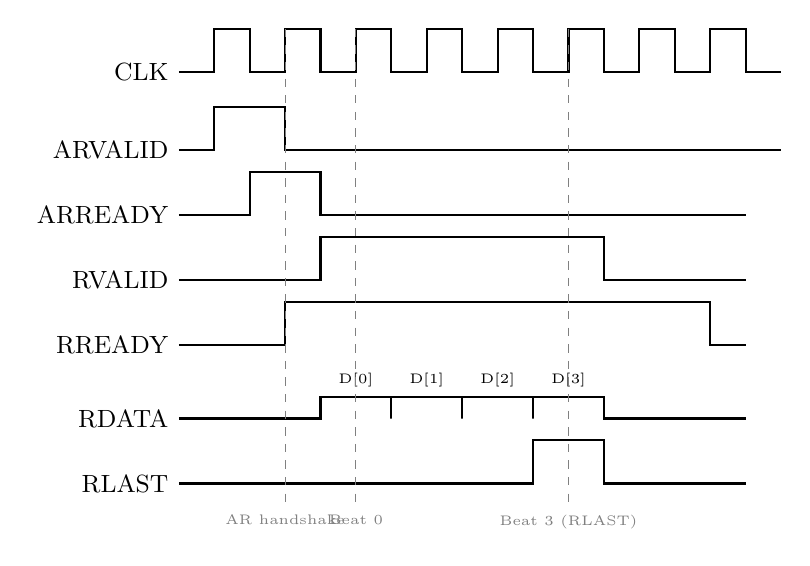
\begin{tikzpicture}[x=0.9cm, y=0.55cm]
  % Clock
  \draw[thick] (0,11) node[left]{\small CLK}
    -- ++(0.5,0)
    foreach \i in {0,...,7}{-- ++(0,1) -- ++(0.5,0) -- ++(0,-1) -- ++(0.5,0)};
  % ARVALID
  \draw[thick] (0,9.2) node[left]{\small ARVALID}
    -- ++(0.5,0) -- ++(0,1) -- ++(1,0) -- ++(0,-1) -- ++(7,0);
  % ARREADY
  \draw[thick] (0,7.7) node[left]{\small ARREADY}
    -- ++(1,0) -- ++(0,1) -- ++(1,0) -- ++(0,-1) -- ++(6,0);
  % RVALID
  \draw[thick] (0,6.2) node[left]{\small RVALID}
    -- ++(2,0) -- ++(0,1) -- ++(4,0) -- ++(0,-1) -- ++(2,0);
  % RREADY
  \draw[thick] (0,4.7) node[left]{\small RREADY}
    -- ++(1.5,0) -- ++(0,1) -- ++(6,0) -- ++(0,-1) -- ++(0.5,0);
  % RDATA beats
  \draw[thick] (0,3) node[left]{\small RDATA}
    -- ++(2,0)
    -- ++(0,0.5) -- ++(1,0) node[midway,above,font=\tiny]{D[0]}
    -- ++(0,-0.5) -- ++(0,0.5) -- ++(1,0) node[midway,above,font=\tiny]{D[1]}
    -- ++(0,-0.5) -- ++(0,0.5) -- ++(1,0) node[midway,above,font=\tiny]{D[2]}
    -- ++(0,-0.5) -- ++(0,0.5) -- ++(1,0) node[midway,above,font=\tiny]{D[3]}
    -- ++(0,-0.5) -- ++(2,0);
  % RLAST
  \draw[thick] (0,1.5) node[left]{\small RLAST}
    -- ++(5,0) -- ++(0,1) -- ++(1,0) -- ++(0,-1) -- ++(2,0);
  % Vertical markers
  \draw[dashed,gray] (1.5,12) -- (1.5,1.0) node[below,font=\tiny]{AR handshake};
  \draw[dashed,gray] (2.5,12) -- (2.5,1.0) node[below,font=\tiny]{Beat 0};
  \draw[dashed,gray] (5.5,12) -- (5.5,1.0) node[below,font=\tiny]{Beat 3 (RLAST)};
\end{tikzpicture}
\caption{AXI4 Cache-Line Fill: 4-Beat INCR Read Burst (ARLEN=3)}
\label{fig:asAxi4Fill}
\end{figure}

\subsubsection{Cache-Line Write-Back Transaction (Write Burst)}

Figure~\ref{fig:asAxi4Wb} shows the timing of a 4-beat INCR write burst
for a D-Cache dirty-line write-back.
The AW and W channels are issued simultaneously.

\begin{figure}[H]
\centering
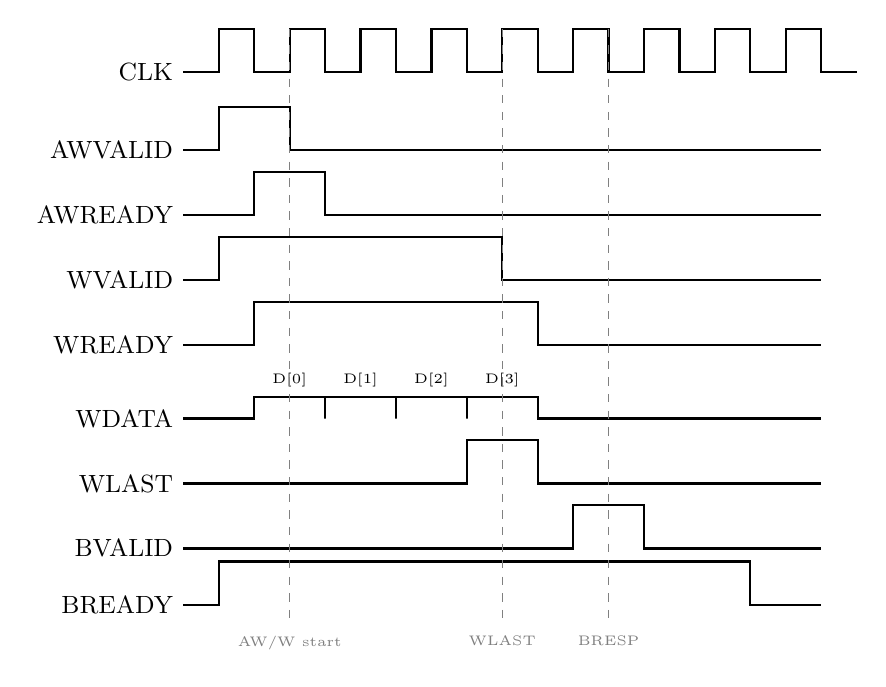
\begin{tikzpicture}[x=0.9cm, y=0.55cm]
  % Clock
  \draw[thick] (0,12) node[left]{\small CLK}
    -- ++(0.5,0)
    foreach \i in {0,...,8}{-- ++(0,1) -- ++(0.5,0) -- ++(0,-1) -- ++(0.5,0)};
  % AWVALID
  \draw[thick] (0,10.2) node[left]{\small AWVALID}
    -- ++(0.5,0) -- ++(0,1) -- ++(1,0) -- ++(0,-1) -- ++(7.5,0);
  % AWREADY
  \draw[thick] (0,8.7) node[left]{\small AWREADY}
    -- ++(1,0) -- ++(0,1) -- ++(1,0) -- ++(0,-1) -- ++(7,0);
  % WVALID
  \draw[thick] (0,7.2) node[left]{\small WVALID}
    -- ++(0.5,0) -- ++(0,1) -- ++(4,0) -- ++(0,-1) -- ++(4.5,0);
  % WREADY
  \draw[thick] (0,5.7) node[left]{\small WREADY}
    -- ++(1,0) -- ++(0,1) -- ++(4,0) -- ++(0,-1) -- ++(4,0);
  % WDATA beats
  \draw[thick] (0,4) node[left]{\small WDATA}
    -- ++(1,0)
    -- ++(0,0.5) -- ++(1,0) node[midway,above,font=\tiny]{D[0]}
    -- ++(0,-0.5) -- ++(0,0.5) -- ++(1,0) node[midway,above,font=\tiny]{D[1]}
    -- ++(0,-0.5) -- ++(0,0.5) -- ++(1,0) node[midway,above,font=\tiny]{D[2]}
    -- ++(0,-0.5) -- ++(0,0.5) -- ++(1,0) node[midway,above,font=\tiny]{D[3]}
    -- ++(0,-0.5) -- ++(4,0);
  % WLAST
  \draw[thick] (0,2.5) node[left]{\small WLAST}
    -- ++(4,0) -- ++(0,1) -- ++(1,0) -- ++(0,-1) -- ++(4,0);
  % BVALID
  \draw[thick] (0,1) node[left]{\small BVALID}
    -- ++(5.5,0) -- ++(0,1) -- ++(1,0) -- ++(0,-1) -- ++(2.5,0);
  % BREADY
  \draw[thick] (0,-0.3) node[left]{\small BREADY}
    -- ++(0.5,0) -- ++(0,1) -- ++(7.5,0) -- ++(0,-1) -- ++(1,0);
  % Markers
  \draw[dashed,gray] (1.5,13) -- (1.5,-0.8) node[below,font=\tiny]{AW/W start};
  \draw[dashed,gray] (4.5,13) -- (4.5,-0.8) node[below,font=\tiny]{WLAST};
  \draw[dashed,gray] (6.0,13) -- (6.0,-0.8) node[below,font=\tiny]{BRESP};
\end{tikzpicture}
\caption{AXI4 Cache Write-Back: 4-Beat INCR Write Burst (AWLEN=3)}
\label{fig:asAxi4Wb}
\end{figure}

%%%%%%%%%%%%%%%%%%%%%%%%%%%%%%%%%%%%%%%%%%%%%%%%%%%%%%%%%%%%%%%%%%%%%%%%%%%%%
\subsection{Memory Arbiter}
%%%%%%%%%%%%%%%%%%%%%%%%%%%%%%%%%%%%%%%%%%%%%%%%%%%%%%%%%%%%%%%%%%%%%%%%%%%%%

\subsubsection{Arbitration Policy}

The Memory Arbiter serialises concurrent AXI4 requests from the I-Cache
and D-Cache controllers onto the single AXI4 port that drives the QSPI
controller.
It implements a \textbf{fixed-priority} scheme with D-Cache having higher
priority than I-Cache.

The rationale is that D-Cache misses in the MEM stage of the pipeline
stall the entire pipeline, while I-Cache misses only stall the IF stage
and can be partially hidden by a deeper instruction buffer in future
pipeline implementations.

\begin{table}[H]
\caption{Memory Arbiter Priority}
\label{tab:asArbPriority}
\centering
\begin{tabularx}{\textwidth}{|l |l |X|}
  \hline
  Priority & Master & Notes \\
  \hline
  \hline
  1 (highest) & D-Cache & Data miss / write-back; stalls the entire pipeline \\
  \hline
  2           & I-Cache & Instruction miss; stalls IF only \\
  \hline
\end{tabularx}
\end{table}

An active transaction is never interrupted: the arbiter grants the bus to
one master for the full burst (ARLEN+1 beats or AWLEN+1 beats) before
switching to the other.

\textbf{Note:} A round-robin policy with equal priority or dynamic priority
based on stall urgency is a future option.

\subsubsection{Memory Arbiter Interface}

\begin{table}[H]
\caption{Memory Arbiter Ports}
\label{tab:asArbPorts}
\centering
\begin{tabularx}{\textwidth}{|l |l |X|}
  \hline
  Port & Type & Description \\
  \hline
  \hline
  \texttt{icache\_axi4} & AXI4 slave  & AXI4 master port of I-Cache controller \\
  \hline
  \texttt{dcache\_axi4} & AXI4 slave  & AXI4 master port of D-Cache controller \\
  \hline
  \texttt{qspi\_axi4}   & AXI4 master & AXI4 slave port of QSPI controller \\
  \hline
\end{tabularx}
\end{table}

The arbiter is purely combinatorial (pass-through mux) for AR, R, AW, W,
and B channels; it adds no pipeline registers.
ID bits from the selected master are forwarded without modification;
the QSPI controller sees only one active ID at a time.

%%%%%%%%%%%%%%%%%%%%%%%%%%%%%%%%%%%%%%%%%%%%%%%%%%%%%%%%%%%%%%%%%%%%%%%%%%%%%
\subsection{QSPI Controller Interface}
%%%%%%%%%%%%%%%%%%%%%%%%%%%%%%%%%%%%%%%%%%%%%%%%%%%%%%%%%%%%%%%%%%%%%%%%%%%%%

The QSPI controller presents an AXI4 slave port to the Memory Arbiter.
From the arbiter's perspective the QSPI controller is a slow memory:
it may de-assert \texttt{ARREADY} / \texttt{WREADY} for many cycles while
the QSPI flash transaction completes.

The cache controllers handle this latency transparently because they hold
\texttt{RREADY} asserted throughout the fill and wait for \texttt{RLAST}
before returning data to the CPU.

\textbf{Note:} The QSPI controller itself is specified in a separate
section of this document.
Its AXI4 slave interface must be compatible with the parameter set in
Table~\ref{tab:asAxi4Params}.
In particular it must support INCR bursts of length 4 (ARLEN=3) at
ARSIZE=3.

%%%%%%%%%%%%%%%%%%%%%%%%%%%%%%%%%%%%%%%%%%%%%%%%%%%%%%%%%%%%%%%%%%%%%%%%%%%%%
\subsection{Cache Flush and Invalidation -- FENCE.I}
\label{subsec:cacheFlush}
%%%%%%%%%%%%%%%%%%%%%%%%%%%%%%%%%%%%%%%%%%%%%%%%%%%%%%%%%%%%%%%%%%%%%%%%%%%%%

\subsubsection{Overview}

A cache flush invalidates all lines in a cache so that subsequent accesses
reload data from the backing store.
In the RWU-RV64I memory architecture, both I-Cache and D-Cache are
\textbf{read-allocate with no write-back}; a flush therefore consists
solely of clearing all \texttt{valid} bits and all PLRU bits in the tag
SRAM.
No dirty eviction is required (MEM-01 resolved).

\subsubsection{Trigger Mechanism}

The flush is triggered by the \textbf{FENCE.I} instruction
(RISC-V Zifencei extension, encoding \texttt{0x0000100F}).
When the instruction decoder recognises FENCE.I it:

\begin{enumerate}
  \item Stalls the CPU pipeline.
  \item Pulses \texttt{ic\_flush\_i} and \texttt{dc\_flush\_i} high for
    one clock cycle.
  \item Waits until both \texttt{ic\_flush\_done\_o} and
    \texttt{dc\_flush\_done\_o} are asserted.
  \item Releases the stall and advances the PC to PC$+4$.
\end{enumerate}

Both caches execute their \texttt{FLUSH} state machines in parallel;
the total stall duration is therefore \textbf{32 clock cycles}
(one write per set, 32 sets).
In a non-pipelined CPU both caches are idle when FENCE.I is decoded,
so no in-flight transaction needs to be drained.

\textbf{No CSR is provided} for cache control; FENCE.I is the sole
software-visible mechanism.
Scratchpad SRAM is not a cache and has no valid bits; it is unaffected
by FENCE.I.

\subsubsection{Flush State Machine}

Both the I-Cache and D-Cache controllers implement an identical
\texttt{FLUSH} state entered when \texttt{*\_flush\_i} is sampled high
in \texttt{IDLE}:

\begin{table}[H]
\caption{FLUSH State -- Operation per Clock Cycle}
\label{tab:asFlushFsm}
\centering
\begin{tabularx}{\textwidth}{|l |X|}
  \hline
  Cycle & Action \\
  \hline
  \hline
  0\ldots30 & Write \texttt{valid[3:0]=4'b0000}, \texttt{plru[2:0]=3'b000}
              to tag SRAM at address \texttt{flush\_cnt[4:0]}; increment
              \texttt{flush\_cnt} \\
  \hline
  31        & Same write for set 31; assert \texttt{*\_flush\_done\_o} for
              one cycle; return to \texttt{IDLE} \\
  \hline
\end{tabularx}
\end{table}

The 5-bit counter \texttt{flush\_cnt} is implemented inside each cache
controller and is reset to zero on entry to \texttt{FLUSH}.
The \texttt{*\_stall\_o} signal remains asserted throughout the 32
cycles and is de-asserted together with \texttt{*\_flush\_done\_o}.

\subsubsection{Software Usage Guidelines}

\begin{itemize}
  \item \textbf{Self-modifying code:} not supported.
    All executable code must reside in NOR Flash; the scratchpad is
    data-only.
    FENCE.I is therefore not required for normal program flow.
  \item \textbf{DMA transfers:} if a future DMA engine writes to the
    Flash address region (e.g.\ via a shadow RAM or XIP staging area),
    the CPU must issue FENCE.I after the DMA completes and before
    executing any updated code.
    See MEM-04 for the coherency protocol.
  \item \textbf{Power-on reset:} both caches initialise with all valid
    bits cleared (reset value of tag SRAM flip-flops); no software flush
    is required at boot.
  \item \textbf{Flush latency:} 32 cycles.
    At a hypothetical 10\,MHz clock (100\,ns cycle) this is 3.2\,\textmu s
    -- negligible for all expected use cases.
\end{itemize}

%%%%%%%%%%%%%%%%%%%%%%%%%%%%%%%%%%%%%%%%%%%%%%%%%%%%%%%%%%%%%%%%%%%%%%%%%%%%%
\subsection{DMA Coherency Protocol}
\label{subsec:dmaCoherency}
%%%%%%%%%%%%%%%%%%%%%%%%%%%%%%%%%%%%%%%%%%%%%%%%%%%%%%%%%%%%%%%%%%%%%%%%%%%%%

\subsubsection{Overview}

A DMA engine transfers data between memory regions without CPU intervention.
Coherency problems arise when the CPU has cached a memory location and the
DMA engine reads or writes that same location, causing one party to see
stale data.

The RWU-RV64I cache architecture minimises DMA coherency complexity through
two structural properties:

\begin{enumerate}
  \item \textbf{Scratchpad is uncacheable.}
    All CPU stores bypass the D-Cache and go directly to the Scratchpad
    SRAM.
    A DMA engine accessing the Scratchpad always sees current data without
    any cache action.
  \item \textbf{D-Cache is read-allocate with no dirty lines.}
    The D-Cache only caches Flash reads.
    Flash is read-only hardware; a DMA engine cannot write to it.
    Therefore the D-Cache can never hold data that is newer than the
    backing store.
\end{enumerate}

\textbf{Recommendation:} place all DMA source and destination buffers in
the Scratchpad address region.
This eliminates every coherency concern at zero hardware cost.

\subsubsection{DMA Access Classification}

Table~\ref{tab:asDmaCoh} enumerates all source/destination combinations
and the required CPU action.

\begin{table}[H]
\caption{DMA Coherency Requirements by Memory Region}
\label{tab:asDmaCoh}
\centering
\begin{tabularx}{\textwidth}{|l |X |X |X|}
  \hline
  DMA source & DMA destination & Coherency issue? & Required CPU action \\
  \hline
  \hline
  Scratchpad & Peripheral & None &
    None. Scratchpad is uncacheable; DMA reads current data. \\
  \hline
  Peripheral & Scratchpad & None &
    None. CPU reads Scratchpad directly; no cache involved. \\
  \hline
  Scratchpad & Scratchpad & None &
    None. Both ends uncacheable. \\
  \hline
  Flash      & Scratchpad & None &
    None. Flash data in D-Cache always matches Flash (read-only). \\
  \hline
  Flash      & Peripheral & None &
    None. As above. \\
  \hline
  Scratchpad & Flash      & N/A  &
    Flash is read-only hardware; this transfer is not possible. \\
  \hline
  Flash      & Flash      & N/A  &
    Flash is read-only hardware as destination; not possible. \\
  \hline
  Peripheral & Flash-mapped cached region\textsuperscript{$\dagger$}
             & \textbf{Yes} &
    CPU must issue \texttt{FENCE.I} \emph{after} DMA completes to
    invalidate stale I-Cache and D-Cache lines. \\
  \hline
\end{tabularx}
\end{table}

\textsuperscript{$\dagger$}Applicable only if a future memory map revision
introduces a writable RAM region within the cacheable address space
(e.g.\ an on-chip SRAM shadow of the Flash area).
In the current architecture this case does not arise.

\subsubsection{Software Protocol}

For the one coherency-relevant scenario (DMA writes to a cacheable region):

\begin{enumerate}
  \item CPU configures the DMA transfer (source, destination, length,
    direction) by writing to DMA control registers (peripheral region,
    uncacheable).
  \item CPU starts the DMA engine and waits for the DMA-done event
    (interrupt or polling of a status register).
  \item CPU issues \texttt{FENCE.I} to invalidate both I-Cache and
    D-Cache (32 cycles).
  \item CPU may now fetch instructions from, or load data out of,
    the DMA-written region; it will see the updated content.
\end{enumerate}

No hardware handshake between the DMA engine and the cache controllers
is required.
The software ordering (wait for DMA done, \emph{then} FENCE.I) is
sufficient because:

\begin{itemize}
  \item The DMA engine writes directly to memory (not through any cache).
  \item FENCE.I invalidates the cache \emph{after} the DMA write is
    visible in memory.
  \item The non-pipelined CPU executes FENCE.I atomically with respect
    to subsequent loads.
\end{itemize}

\subsubsection{Future DMA Engine Interface Requirements}

When the DMA engine is designed, it must expose at minimum:

\begin{table}[H]
\caption{Minimum DMA Engine Signals for Cache Coherency}
\label{tab:asDmaIf}
\centering
\begin{tabularx}{\textwidth}{|l |l |X|}
  \hline
  Signal & Type & Purpose \\
  \hline
  \hline
  \texttt{dma\_done\_irq} & out (to CPU) &
    Interrupt asserted when DMA transfer completes; CPU uses this as the
    trigger to issue \texttt{FENCE.I} before accessing DMA-written data \\
  \hline
  \texttt{dma\_active\_o} & out (to system) &
    High while a transfer is in progress; optional, used to prevent
    conflicting CPU accesses to the same address range \\
  \hline
\end{tabularx}
\end{table}

No cache-flush or cache-snoop signal is required from the DMA engine;
the software protocol (Section above) is sufficient.

%%%%%%%%%%%%%%%%%%%%%%%%%%%%%%%%%%%%%%%%%%%%%%%%%%%%%%%%%%%%%%%%%%%%%%%%%%%%%
\subsection{AXI4 Error Handling}
\label{subsec:axi4Error}
%%%%%%%%%%%%%%%%%%%%%%%%%%%%%%%%%%%%%%%%%%%%%%%%%%%%%%%%%%%%%%%%%%%%%%%%%%%%%

\subsubsection{Overview}

The AXI4 read response channel (\texttt{RRESP[1:0]}) carries a completion
status from the QSPI controller back to the cache controllers.
A non-OKAY response indicates that the underlying NOR Flash transaction
failed (e.g.\ timeout, command error, or address out of Flash range).

In the RWU-RV64I design the AXI4 write channels (AW, W, B) are eliminated
from the cache controllers (MEM-01); \texttt{BRESP} is therefore not
observed and requires no handling.

AXI4 errors are surfaced to software as standard
\textbf{RISC-V Machine-Mode Exceptions} following the Privileged
Architecture specification.
This is the correct approach: the CPU already has exception infrastructure
(for illegal instructions, etc.) and the trap handler can log, retry, or
halt in a well-defined way.

\subsubsection{AXI4 Response Codes}

\begin{table}[H]
\caption{AXI4 RRESP Codes Handled by Cache Controllers}
\label{tab:asRresp}
\centering
\begin{tabularx}{\textwidth}{|l |l |l |X|}
  \hline
  \texttt{RRESP} & Name & Used? & Action \\
  \hline
  \hline
  2'b00 & OKAY   & Yes & Normal completion; data written to cache SRAM \\
  \hline
  2'b01 & EXOKAY & No  & Exclusive access OK; not used (no LR/SC in this design) \\
  \hline
  2'b10 & SLVERR & Yes & Slave error (QSPI / Flash fault); triggers exception \\
  \hline
  2'b11 & DECERR & Yes & Decode error (address unmapped); triggers exception \\
  \hline
\end{tabularx}
\end{table}

\subsubsection{Exception Mapping}

Table~\ref{tab:asAxi4Exc} maps AXI4 error events to RISC-V exception
causes.

\begin{table}[H]
\caption{AXI4 Error to RISC-V Exception Mapping}
\label{tab:asAxi4Exc}
\centering
\begin{tabularx}{\textwidth}{|l |l |l |X |X|}
  \hline
  Cache & AXI4 signal & \texttt{mcause} & Exception name & \texttt{mtval} \\
  \hline
  \hline
  I-Cache & \texttt{RRESP} $\neq$ OKAY & 1 & Instruction Access Fault &
    Faulting fetch address (\texttt{ic\_addr\_i} at time of miss) \\
  \hline
  D-Cache & \texttt{RRESP} $\neq$ OKAY & 5 & Load Access Fault &
    Faulting load address (\texttt{dc\_addr\_i} at time of miss) \\
  \hline
\end{tabularx}
\end{table}

\subsubsection{Error Detection in the Cache Controllers}

Both cache controllers monitor \texttt{RRESP} on every beat of the R
channel during the \texttt{FILL} state.
If any beat carries \texttt{RRESP} $\neq$ \texttt{2'b00}:

\begin{enumerate}
  \item The cache controller immediately stops writing to the data SRAM.
  \item The valid bit for the partially filled line is \textbf{not} set
    (the line remains invalid).
  \item The controller transitions to the new \texttt{ERR} state.
  \item In \texttt{ERR}, the controller pulses the error output
    (\texttt{ic\_err\_o} or \texttt{dc\_err\_o}) for one cycle and
    asserts the corresponding stall signal for that cycle.
  \item The controller returns to \texttt{IDLE}.
\end{enumerate}

The CPU samples the error output on the same cycle as the stall
de-assertion, latches the faulting address, and raises the appropriate
exception.

\subsubsection{Updated Cache Controller FSMs}

The \texttt{ERR} state is added to both I-Cache and D-Cache FSMs.

\begin{table}[H]
\caption{ERR State -- I-Cache and D-Cache (identical behaviour)}
\label{tab:asErrState}
\centering
\begin{tabularx}{\textwidth}{|l |X|}
  \hline
  Condition & Action \\
  \hline
  \hline
  Entry condition &
    Any AXI4 R-channel beat with \texttt{RRESP} $\neq$ \texttt{2'b00}
    during \texttt{FILL} \\
  \hline
  In \texttt{ERR} (1 cycle) &
    Do not update tag SRAM valid bit.
    Assert \texttt{*\_err\_o} for one cycle.
    Assert \texttt{*\_stall\_o} for the same cycle. \\
  \hline
  Exit condition &
    Unconditional; return to \texttt{IDLE} after one cycle \\
  \hline
\end{tabularx}
\end{table}

\subsubsection{Updated Cache Interface Signals}

One error output signal is added to each cache interface.

\begin{table}[H]
\caption{Error Signals Added to Cache Interfaces}
\label{tab:asErrSig}
\centering
\begin{tabularx}{\textwidth}{|l |l |l |l |X|}
  \hline
  Signal & Interface & Dir (CPU) & Width & Description \\
  \hline
  \hline
  \texttt{ic\_err\_o} & \texttt{as\_icache\_if} & in & 1 &
    Pulsed high for one cycle on an I-Cache AXI4 read error;
    CPU raises Instruction Access Fault (\texttt{mcause}=1) \\
  \hline
  \texttt{dc\_err\_o} & \texttt{as\_dcache\_if} & in & 1 &
    Pulsed high for one cycle on a D-Cache AXI4 read error;
    CPU raises Load Access Fault (\texttt{mcause}=5) \\
  \hline
\end{tabularx}
\end{table}

\subsubsection{CPU Exception Handling Sequence}

When the CPU samples \texttt{ic\_err\_o} or \texttt{dc\_err\_o}:

\begin{enumerate}
  \item Save the current PC to \texttt{mepc}.
  \item Write the exception cause to \texttt{mcause}
    (1 for I-Cache, 5 for D-Cache).
  \item Write the faulting address to \texttt{mtval}
    (last value driven on \texttt{ic\_addr\_i} or \texttt{dc\_addr\_i}).
  \item Clear \texttt{mstatus.MIE} (disable interrupts).
  \item Jump to \texttt{mtvec} (trap vector).
\end{enumerate}

The trap handler at \texttt{mtvec} may:

\begin{itemize}
  \item \textbf{Halt:} for a non-recoverable Flash fault this is the
    correct default action (e.g.\ output error code via UART/GPIO,
    then \texttt{wfi}).
  \item \textbf{Retry:} re-execute the faulting instruction
    (\texttt{mret} after optionally re-initialising the QSPI controller).
    Appropriate for transient QSPI timeouts.
  \item \textbf{Substitute:} fill a scratchpad buffer with alternative
    data, remap the faulting address (if an MPU is present), and
    \texttt{mret}.
    Advanced; not required for the first tapeout.
\end{itemize}

\subsubsection{Updated SystemVerilog Interfaces}

\begin{verbatim}
// as_icache_if additions:
logic ic_err;       // new: AXI4 read error → Instruction Access Fault
modport cpu  (..., input ic_err);
modport cache(..., output ic_err);

// as_dcache_if additions:
logic dc_err;       // new: AXI4 read error → Load Access Fault
modport cpu  (..., input dc_err);
modport cache(..., output dc_err);
\end{verbatim}

Full updated interface definitions are in
Sections~\ref{subsec:iBusIf} and~\ref{subsec:dBusIf}.

%%%%%%%%%%%%%%%%%%%%%%%%%%%%%%%%%%%%%%%%%%%%%%%%%%%%%%%%%%%%%%%%%%%%%%%%%%%%%
\subsection{QSPI Operating Mode -- Cache-Miss-Driven Read}
\label{subsec:qspiMode}
%%%%%%%%%%%%%%%%%%%%%%%%%%%%%%%%%%%%%%%%%%%%%%%%%%%%%%%%%%%%%%%%%%%%%%%%%%%%%

\subsubsection{XIP Terminology Clarification}

The term \emph{Execute-In-Place} (XIP) is used with two distinct meanings
in the literature:

\begin{itemize}
  \item \textbf{True XIP (Continuous Read mode):} the QSPI controller
    keeps the Flash chip-select asserted and the device in a special
    Continuous Read state; subsequent reads require only the address
    (no repeated opcode), reducing per-transaction overhead.
    Requires the Flash to support a Performance Enhance or XIP mode bit.
  \item \textbf{Indirect XIP (cache-miss-driven):} the CPU executes code
    that resides in Flash, but each cache miss triggers a complete SPI
    command sequence (opcode + address + dummy + data).
    The chip-select is asserted only for the duration of each burst.
    No special Flash mode is required.
\end{itemize}

\textbf{Decision:} the RWU-RV64I uses \textbf{indirect XIP}
(cache-miss-driven burst mode).
True XIP mode is neither necessary nor advantageous for this architecture,
as explained below.

\subsubsection{Rationale}

True XIP mode is not adopted for the following reasons:

\begin{enumerate}
  \item \textbf{The I-Cache already provides the XIP benefit.}
    Once a cache line is loaded, all subsequent accesses to it cost 1
    clock cycle.
    The amortised QSPI overhead per instruction is negligible at
    realistic hit rates ($>$90\,\%).
  \item \textbf{Sequential access is not guaranteed.}
    A 4-way set-associative cache evicts and reloads lines at
    non-sequential addresses.
    True XIP's main advantage (no repeated opcode/address) applies
    only to sequential reads; for random-address cache refills its
    benefit is minimal.
  \item \textbf{Simpler QSPI controller.}
    Indirect XIP requires no Flash-mode-bit management, no
    continuous-read entry/exit sequence, and no special handling for
    the transition back from XIP mode (required before write/erase
    operations in True XIP).
  \item \textbf{Lower power between cache misses.}
    With CS\# de-asserted between bursts the Flash enters standby
    mode automatically, reducing leakage current.
\end{enumerate}

\subsubsection{QSPI Command Sequence per Cache Miss}

On each cache miss the QSPI controller executes the following sequence
on the SPI bus:

\begin{enumerate}
  \item Assert CS\# (chip select, active-low).
  \item Send read opcode on IO0 (single-bit SPI).
  \item Send 24-bit (3-byte) Flash address on IO0; address is taken
    directly from \texttt{ARADDR[24:0]} (for Flash devices up to 16\,MB)
    or \texttt{ARADDR[31:0]} for larger devices.
    The lower 5 bits are always zero (cache-line aligned burst).
  \item Send dummy cycles (device-specific; typically 8 clock cycles
    for Fast Read, 6--8 for Quad Fast Read).
  \item Receive 32 bytes of read data, output on IO0 (Fast Read) or
    IO0--IO3 simultaneously (Quad Fast Read).
    Data is returned to the AXI4 R channel as 4 beats of 64 bits,
    LSB-first within each beat.
  \item De-assert CS\#.
\end{enumerate}

\begin{table}[H]
\caption{Supported QSPI Read Commands}
\label{tab:asQspiCmd}
\centering
\begin{tabularx}{\textwidth}{|l |l |l |l |X|}
  \hline
  Command & Opcode & Mode & Throughput & Notes \\
  \hline
  \hline
  Fast Read        & \texttt{0x0B} & 1-bit SPI  & Low    &
    Fallback; maximum QSPI clock limited by Flash spec \\
  \hline
  Quad Fast Read   & \texttt{0x6B} & 4-bit QSPI & High   &
    \textbf{Recommended}; data on IO0--IO3 in parallel;
    requires QUAD enable bit set in Flash status register \\
  \hline
\end{tabularx}
\end{table}

The Quad Fast Read command (\texttt{0x6B}) is recommended because it
reduces the data phase from 256 QSPI clock cycles (single-bit) to
64 QSPI clock cycles (four-bit), significantly lowering cache-miss
latency.

\subsubsection{Address Mapping}

The AXI4 \texttt{ARADDR} is used directly as the Flash physical address:

\[
  \texttt{Flash\_Addr}[24:5] = \texttt{ARADDR}[24:5], \quad
  \texttt{Flash\_Addr}[4:0] = 5'b00000
\]

The five least-significant address bits are always zero because the
cache controller aligns all burst requests to the 32-byte cache-line
boundary before issuing the AXI4 transaction.

\subsubsection{Latency Estimate}

Table~\ref{tab:asQspiLat} estimates the QSPI bus cycles and system
clock cycles consumed by a single cache-line fill using Quad Fast Read.
Actual values depend on the Flash device datasheet and the QSPI clock
divider setting.

\begin{table}[H]
\caption{Cache-Line Fill Latency Estimate (Quad Fast Read, \texttt{0x6B})}
\label{tab:asQspiLat}
\centering
\begin{tabularx}{\textwidth}{|l |l |X|}
  \hline
  Phase & QSPI clocks & Notes \\
  \hline
  \hline
  CS\# assert + opcode  &  8 & 8-bit opcode on IO0 \\
  \hline
  Address               & 24 & 24-bit address on IO0 \\
  \hline
  Dummy cycles          &  8 & Device-specific; 8 typical for \texttt{0x6B} \\
  \hline
  Data (32\,bytes)      & 64 & 256 bits $\div$ 4 (quad) = 64 QSPI clocks \\
  \hline
  CS\# de-assert        &  2 & Minimum CS\# high time (device-specific) \\
  \hline
  \textbf{Total}        & \textbf{106} & Per cache miss \\
  \hline
\end{tabularx}
\end{table}

At an example QSPI clock of 25\,MHz and system clock of 10\,MHz:
\[
  t_\text{miss} = \frac{106}{25\,\text{MHz}} = 4.24\,\mu\text{s}
  \;\widehat{=}\; 42\;\text{system clock cycles}.
\]
This is consistent with the ``$\gg$10 cycles'' estimate in
Table~\ref{tab:asMemHierarchy}.
The exact QSPI clock frequency and divider ratio are to be determined
once the target NOR Flash device is selected.

\subsubsection{NOR Flash Device Requirements}

The selected NOR Flash must support:

\begin{itemize}
  \item \textbf{Quad Fast Read (0x6B)} with up to 8 dummy cycles.
  \item \textbf{3-byte address mode} (24-bit, supports Flash up to 16\,MB);
    or 4-byte mode if a larger device is required.
  \item \textbf{AXI4 burst compatibility:} the device must sustain
    continuous 4-bit output for 64 QSPI clocks without inserting wait
    states.
  \item \textbf{3.3\,V supply} (matching XO035 I/O voltage).
\end{itemize}

%%%%%%%%%%%%%%%%%%%%%%%%%%%%%%%%%%%%%%%%%%%%%%%%%%%%%%%%%%%%%%%%%%%%%%%%%%%%%
\subsection{Memory Hierarchy Performance Analysis}
\label{subsec:memPerfAnalysis}
%%%%%%%%%%%%%%%%%%%%%%%%%%%%%%%%%%%%%%%%%%%%%%%%%%%%%%%%%%%%%%%%%%%%%%%%%%%%%

\subsubsection{Average Memory Access Time (AMAT)}

The standard metric for cache hierarchy performance is the
\textbf{Average Memory Access Time (AMAT)}:

\[
  \text{AMAT} = t_\text{hit} + m_1 \cdot t_\text{miss}
\]

where $t_\text{hit}$ is the cache hit latency, $m_1$ is the L1 miss rate,
and $t_\text{miss}$ is the miss penalty.
For the current two-level hierarchy (L1 cache + NOR Flash) the values
from this document are:

\begin{itemize}
  \item $t_\text{hit} = 1$ cycle (cache hit, combinatorial tag compare +
        SRAM read).
  \item $t_\text{miss} = 42$ system clock cycles (cache-line fill from
        NOR Flash via QSPI Quad Fast Read at 25\,MHz QSPI /
        10\,MHz system; see Table~\ref{tab:asQspiLat}).
\end{itemize}

Thus:
\[
  \text{AMAT}_\text{2-level} = 1 + m_1 \cdot 42 \quad \text{[system cycles]}
\]

\subsubsection{Hypothetical Three-Level Hierarchy}

If an additional on-chip SRAM layer (L2) were inserted between the L1
caches and NOR Flash, the AMAT becomes:

\[
  \text{AMAT}_\text{3-level} = 1 + m_1 \cdot \bigl(t_\text{L2} + m_2 \cdot 42\bigr)
\]

where $t_\text{L2}$ is the L2 SRAM access time (1--2 cycles for an
on-chip synchronous SRAM) and $m_2$ is the fraction of L1 misses that
also miss in L2.
The resulting speed-up $S = \text{AMAT}_\text{2-level} /
\text{AMAT}_\text{3-level}$ is shown in
Table~\ref{tab:asMemSpeedup}.

\begin{table}[H]
\caption{AMAT and Speed-Up for a Hypothetical L2 SRAM
         ($t_\text{L2} = 2$ cycles, $t_\text{miss} = 42$ cycles)}
\label{tab:asMemSpeedup}
\centering
\begin{tabularx}{\textwidth}{|l |l |l |l |l|}
  \hline
  L1 miss rate $m_1$ & L2 miss rate $m_2$ & AMAT$_\text{2-level}$ &
  AMAT$_\text{3-level}$ & Speed-Up \\
  \hline
  \hline
  5\,\%  & 0\,\% (program fits in L2)  & 3.1 & 1.10 & $2.8\times$ \\
  \hline
  10\,\% & 0\,\%                       & 5.2 & 1.20 & $4.3\times$ \\
  \hline
  20\,\% & 0\,\%                       & 9.4 & 1.40 & $6.7\times$ \\
  \hline
  10\,\% & 20\,\% (L2 80\,\% hit rate) & 5.2 & 2.04 & $2.5\times$ \\
  \hline
  10\,\% & 50\,\%                       & 5.2 & 3.10 & $1.7\times$ \\
  \hline
\end{tabularx}
\end{table}

The maximum benefit occurs when the active working set fits entirely
in L2 ($m_2 \approx 0\,\%$), in which case NOR Flash is accessed only
during the initial boot load and AMAT approaches $1 + m_1 \cdot t_\text{L2}$.

\subsubsection{System-Clock Scaling of the Miss Penalty}

The QSPI transaction consumes a \emph{fixed number of QSPI clock cycles}
(106 at 25\,MHz QSPI; see Table~\ref{tab:asQspiLat}).
Converting to system clock cycles:

\[
  t_\text{miss}[\text{sys}] = \frac{106}{f_\text{QSPI}} \cdot f_\text{sys}
  = 106 \cdot \frac{f_\text{sys}}{f_\text{QSPI}}
\]

\begin{table}[H]
\caption{Miss Penalty vs.\ System Clock (QSPI fixed at 25\,MHz)}
\label{tab:asQspiMissPenaltyScaling}
\centering
\begin{tabularx}{\textwidth}{|l |l |l |X|}
  \hline
  System clock & QSPI clock & Miss penalty & Remark \\
  \hline
  \hline
  10\,MHz & 25\,MHz & 42 cycles  & Reference design point \\
  \hline
  25\,MHz & 25\,MHz & 106 cycles & Penalty $2.5\times$ longer \\
  \hline
  50\,MHz & 25\,MHz & 212 cycles & Penalty $5\times$ longer \\
  \hline
\end{tabularx}
\end{table}

The penalty in system cycles grows linearly with the system clock when
the QSPI clock is held constant.
An additional on-chip SRAM layer therefore becomes increasingly
beneficial as the system clock is raised.

\subsubsection{Design Decision}
\label{subsubsec:l2Decision}

The current architecture intentionally omits an L2 cache layer:

\begin{itemize}
  \item \textbf{Chip area:} At X-Fab XO035 (350\,nm) a true L2 cache
    (tag array, replacement logic, coherency protocol) consumes
    significant die area.
  \item \textbf{Complexity:} An L2 controller adds coherency and
    arbitration logic on top of the existing Memory Arbiter.
  \item \textbf{Scratchpad covers the critical path:}
    Stack, heap, \texttt{.data}, and \texttt{.bss} reside in the
    Scratchpad SRAM (1--2 cycle access); these are the write-intensive
    segments that would most benefit from low latency.
    Only code (\texttt{.text}) and read-only data (\texttt{.rodata})
    remain in the Flash/cache path.
  \item \textbf{4\,KB L1 miss rate:} For small embedded programs that
    fit in the 4\,KB I-Cache, the instruction miss rate is low after
    the initial cache warm-up, limiting the absolute time spent on
    Flash accesses.
\end{itemize}

Should the system clock be raised significantly above 10\,MHz or should
larger programs with a high L1 miss rate become a requirement, adding a
Tightly Coupled Memory (TCM) layer -- an on-chip SRAM preloaded from
Flash at boot -- would be the recommended approach.
A full L2 cache is not recommended for the first tape-out on this
process node.

%%%%%%%%%%%%%%%%%%%%%%%%%%%%%%%%%%%%%%%%%%%%%%%%%%%%%%%%%%%%%%%%%%%%%%%%%%%%%
\subsection{SystemVerilog Module Architecture}
\label{subsec:svModules}
%%%%%%%%%%%%%%%%%%%%%%%%%%%%%%%%%%%%%%%%%%%%%%%%%%%%%%%%%%%%%%%%%%%%%%%%%%%%%

This section specifies the SystemVerilog module decomposition of the
memory subsystem.
Each module is described with its complete port list (signal, direction,
width, connected to/from, and purpose) and its internal algorithm.
The module names follow the project-wide \texttt{as} prefix convention.

\subsubsection{Module Hierarchy}
\label{subsubsec:modHierarchy}

Table~\ref{tab:asModHierarchy} lists all modules.
\texttt{asMemTop} is the sole instantiation point; the CPU core and the
QSPI controller are outside this boundary.

\begin{table}[H]
\caption{Memory Subsystem -- SystemVerilog Module Overview}
\label{tab:asModHierarchy}
\centering
\begin{tabularx}{\textwidth}{|l |l |X|}
  \hline
  Module & Type & Purpose \\
  \hline
  \hline
  \texttt{asMemTop}      & top wrapper   & Instantiates all sub-modules; routes CPU, SRAM and AXI4 interfaces \\
  \hline
  \texttt{asICacheCtrl}  & RTL (FSM)     & Instruction cache controller: tag compare, PLRU, AXI4 master (AR/R) \\
  \hline
  \texttt{asDCacheCtrl}  & RTL (FSM)     & Data cache controller: tag compare, PLRU, bypass path, AXI4 master (AR/R) \\
  \hline
  \texttt{asICacheBlock} & SRAM wrapper  & Holds I-Tag SRAM (96\,bit$\times$32) and I-Data SRAM (256\,bit$\times$128) \\
  \hline
  \texttt{asDCacheBlock} & SRAM wrapper  & Holds D-Tag SRAM (96\,bit$\times$32) and D-Data SRAM (256\,bit$\times$128) \\
  \hline
  \texttt{asSpBlock}     & SRAM wrapper  & Holds Scratchpad SRAM (64\,bit$\times$1024) \\
  \hline
  \texttt{asMemArb}      & RTL (mux)     & Fixed-priority AXI4 arbiter: D-Cache\,$>$\,I-Cache, single output port \\
  \hline
  \texttt{asSpramModel}  & sim. model    & Behavioural 1-cycle synchronous SRAM; replaces X-Fab SPRAM macro in simulation \\
  \hline
\end{tabularx}
\end{table}

The three SRAM wrapper modules (\texttt{asICacheBlock}, \texttt{asDCacheBlock},
\texttt{asSpBlock}) each instantiate one or two X-Fab XO035 SPRAM macros.
In simulation the macros are replaced by \texttt{asSpramModel} via a
synthesis guard (\texttt{`ifdef SIMULATION}).

% -------------------------------------------------------------------------
\subsubsection{\texttt{asMemTop} -- Memory Subsystem Top}
\label{subsubsec:asMemTop}

\paragraph{Purpose.}
Top-level wrapper that wires the CPU interfaces, the SRAM blocks, the
cache controllers, and the memory arbiter together.
It presents three external interfaces: the CPU instruction bus, the CPU
data bus, and the AXI4 master port toward the QSPI controller.
No combinatorial or sequential logic resides in this module beyond
wire connections and interface bindings.

\paragraph{Port list.}

\begin{table}[H]
\caption{\texttt{asMemTop} Port List}
\label{tab:asMemTopPorts}
\centering
\begin{tabularx}{\textwidth}{|l |l |l |l |X|}
  \hline
  Signal & Dir & Width & Connected to & Description \\
  \hline
  \hline
  \multicolumn{5}{|l|}{\textit{Clock and Reset}} \\
  \hline
  \texttt{clk\_i}  & in & 1 & All sub-modules & System clock (synchronous rising edge) \\
  \hline
  \texttt{rst\_i}  & in & 1 & All sub-modules & Synchronous active-high reset \\
  \hline
  \multicolumn{5}{|l|}{\textit{CPU Instruction Bus (via \texttt{as\_icache\_if})}} \\
  \hline
  \texttt{ic\_addr\_i}        & in  & 64 & \texttt{asICacheCtrl} & Fetch address from CPU IF stage \\
  \hline
  \texttt{ic\_req\_i}         & in  & 1  & \texttt{asICacheCtrl} & Fetch request valid \\
  \hline
  \texttt{ic\_flush\_i}       & in  & 1  & \texttt{asICacheCtrl} & FENCE.I pulse from CPU \\
  \hline
  \texttt{ic\_stall\_o}       & out & 1  & CPU IF stage          & Cache miss / flush in progress \\
  \hline
  \texttt{ic\_flush\_done\_o} & out & 1  & CPU IF stage          & Flush complete pulse \\
  \hline
  \texttt{ic\_err\_o}         & out & 1  & CPU IF stage          & AXI4 read error pulse \\
  \hline
  \texttt{ic\_rdata\_o}       & out & 32 & CPU IF stage          & Instruction word (32-bit) \\
  \hline
  \texttt{ic\_rvalid\_o}      & out & 1  & CPU IF stage          & Instruction word valid \\
  \hline
  \multicolumn{5}{|l|}{\textit{CPU Data Bus (via \texttt{as\_dcache\_if})}} \\
  \hline
  \texttt{dc\_addr\_i}        & in  & 64 & \texttt{asDCacheCtrl} & Load/store address from CPU MEM stage \\
  \hline
  \texttt{dc\_req\_i}         & in  & 1  & \texttt{asDCacheCtrl} & Load/store request valid \\
  \hline
  \texttt{dc\_wr\_i}          & in  & 1  & \texttt{asDCacheCtrl} & 1\,=\,store, 0\,=\,load \\
  \hline
  \texttt{dc\_size\_i}        & in  & 3  & \texttt{asDCacheCtrl} & Transfer size (byte/half/word/double) \\
  \hline
  \texttt{dc\_wdata\_i}       & in  & 64 & \texttt{asDCacheCtrl} & Store data from CPU \\
  \hline
  \texttt{dc\_wstrb\_i}       & in  & 8  & \texttt{asDCacheCtrl} & Byte enables for store \\
  \hline
  \texttt{dc\_flush\_i}       & in  & 1  & \texttt{asDCacheCtrl} & FENCE.I pulse from CPU \\
  \hline
  \texttt{dc\_stall\_o}       & out & 1  & CPU MEM stage         & Cache miss / bypass / flush in progress \\
  \hline
  \texttt{dc\_flush\_done\_o} & out & 1  & CPU MEM stage         & Flush complete pulse \\
  \hline
  \texttt{dc\_err\_o}         & out & 1  & CPU MEM stage         & AXI4 read error pulse \\
  \hline
  \texttt{dc\_rdata\_o}       & out & 64 & CPU MEM stage         & Load data (64-bit) \\
  \hline
  \texttt{dc\_rvalid\_o}      & out & 1  & CPU MEM stage         & Load data valid \\
  \hline
  \multicolumn{5}{|l|}{\textit{AXI4 Master Port toward QSPI Controller (via \texttt{as\_axi4\_if})}} \\
  \hline
  \texttt{m\_axi4}            & out & -- & \texttt{asQspiTop}    & AXI4 master bundle (AR, R channels only; see Table~\ref{tab:asAxi4Params}) \\
  \hline
\end{tabularx}
\end{table}

\paragraph{Internal algorithm.}
\texttt{asMemTop} contains no logic.
It instantiates exactly the seven modules listed in
Table~\ref{tab:asModHierarchy} (excluding \texttt{asSpramModel}, which
lives inside the SRAM wrappers) and connects them via the SV interfaces
\texttt{as\_icache\_if}, \texttt{as\_dcache\_if}, and \texttt{as\_axi4\_if}.
The SRAM wrappers are wired to their respective controllers through
dedicated flat port groups (see Sections~\ref{subsubsec:asICacheBlock}
through~\ref{subsubsec:asSpBlock}).

% -------------------------------------------------------------------------
\subsubsection{\texttt{asICacheBlock} -- I-Cache SRAM Wrapper}
\label{subsubsec:asICacheBlock}

\paragraph{Purpose.}
Wraps two X-Fab XO035 SPRAM macros: the I-Tag SRAM (96\,bit\,$\times$\,32)
and the I-Data SRAM (256\,bit\,$\times$\,128).
Translates the logical controller signals into the physical SPRAM port
signals (\texttt{CLK}, \texttt{CEN}, \texttt{WEN}, \texttt{BWEN},
\texttt{A}, \texttt{D}, \texttt{Q}) described in
Section~\ref{subsec:sramMacros}.
In simulation the SPRAM macros are replaced by \texttt{asSpramModel}.

\paragraph{Port list.}

\begin{table}[H]
\caption{\texttt{asICacheBlock} Port List}
\label{tab:asICacheBlockPorts}
\centering
\begin{tabularx}{\textwidth}{|l |l |l |l |X|}
  \hline
  Signal & Dir & Width & Connected to & Description \\
  \hline
  \hline
  \texttt{clk\_i}         & in  & 1   & SPRAM CLK         & System clock \\
  \hline
  \multicolumn{5}{|l|}{\textit{Tag SRAM port (I-Tag SRAM, 96\,bit\,$\times$\,32)}} \\
  \hline
  \texttt{it\_addr\_i}    & in  & 5   & \texttt{asICacheCtrl} & Set index (0--31) \\
  \hline
  \texttt{it\_wdata\_i}   & in  & 96  & \texttt{asICacheCtrl} & Tag write data: \{PLRU[2:0], way3\{valid,tag[21:0]\}, \ldots, way0\{valid,tag[21:0]\}\} \\
  \hline
  \texttt{it\_we\_i}      & in  & 1   & \texttt{asICacheCtrl} & Tag write enable (active-high) \\
  \hline
  \texttt{it\_ce\_i}      & in  & 1   & \texttt{asICacheCtrl} & Tag chip enable (active-high) \\
  \hline
  \texttt{it\_rdata\_o}   & out & 96  & \texttt{asICacheCtrl} & Tag read data; valid one cycle after \texttt{it\_ce\_i} on read \\
  \hline
  \multicolumn{5}{|l|}{\textit{Data SRAM port (I-Data SRAM, 256\,bit\,$\times$\,128)}} \\
  \hline
  \texttt{id\_addr\_i}    & in  & 7   & \texttt{asICacheCtrl} & Address: \{index[4:0], way[1:0]\} \\
  \hline
  \texttt{id\_wdata\_i}   & in  & 64  & \texttt{asICacheCtrl} & One 64-bit beat to write; placed into the lane selected by \texttt{id\_wlane\_i} \\
  \hline
  \texttt{id\_wlane\_i}   & in  & 2   & \texttt{asICacheCtrl} & Beat index (0--3); selects 64-bit lane within 256-bit word \\
  \hline
  \texttt{id\_we\_i}      & in  & 1   & \texttt{asICacheCtrl} & Data write enable (active-high) \\
  \hline
  \texttt{id\_ce\_i}      & in  & 1   & \texttt{asICacheCtrl} & Data chip enable (active-high) \\
  \hline
  \texttt{id\_rdata\_o}   & out & 256 & \texttt{asICacheCtrl} & Full 256-bit cache line; valid one cycle after \texttt{id\_ce\_i} on read \\
  \hline
\end{tabularx}
\end{table}

\paragraph{Internal algorithm.}
On a write (\texttt{it\_we\_i} or \texttt{id\_we\_i} high):
\begin{itemize}
  \item Tag SRAM: \texttt{BWEN} is set to all-zero (write all 96 bits);
    \texttt{WEN} is driven low; \texttt{A} receives \texttt{it\_addr\_i};
    \texttt{D} receives \texttt{it\_wdata\_i}.
  \item Data SRAM: \texttt{id\_wlane\_i} selects one 64-bit lane.
    \texttt{BWEN[255:0]} is constructed as: bits\,$[(lane+1)\cdot64-1\,:\,lane\cdot64]$
    are driven to \texttt{0} (write-enable); all other bits are \texttt{1}
    (mask).
    \texttt{D[63:0]} is replicated four times to fill \texttt{D[255:0]};
    only the selected lane is actually written due to BWEN masking.
\end{itemize}
On a read (\texttt{it\_ce\_i} or \texttt{id\_ce\_i} high, write enables
low): \texttt{WEN} is driven high; \texttt{BWEN} is irrelevant (ignored
on reads by the SPRAM); the read data appears on \texttt{Q} one clock
cycle later.

% -------------------------------------------------------------------------
\subsubsection{\texttt{asDCacheBlock} -- D-Cache SRAM Wrapper}
\label{subsubsec:asDCacheBlock}

\paragraph{Purpose.}
Identical in structure to \texttt{asICacheBlock} but serves the D-Cache
controller.
Wraps D-Tag SRAM (96\,bit\,$\times$\,32) and D-Data SRAM
(256\,bit\,$\times$\,128); same SPRAM macros, same timing, same
simulation guard.

\paragraph{Port list.}

\begin{table}[H]
\caption{\texttt{asDCacheBlock} Port List}
\label{tab:asDCacheBlockPorts}
\centering
\begin{tabularx}{\textwidth}{|l |l |l |l |X|}
  \hline
  Signal & Dir & Width & Connected to & Description \\
  \hline
  \hline
  \texttt{clk\_i}         & in  & 1   & SPRAM CLK             & System clock \\
  \hline
  \multicolumn{5}{|l|}{\textit{Tag SRAM port (D-Tag SRAM, 96\,bit\,$\times$\,32)}} \\
  \hline
  \texttt{dt\_addr\_i}    & in  & 5   & \texttt{asDCacheCtrl} & Set index (0--31) \\
  \hline
  \texttt{dt\_wdata\_i}   & in  & 96  & \texttt{asDCacheCtrl} & Tag write data (same layout as I-Cache; no dirty bit) \\
  \hline
  \texttt{dt\_we\_i}      & in  & 1   & \texttt{asDCacheCtrl} & Tag write enable (active-high) \\
  \hline
  \texttt{dt\_ce\_i}      & in  & 1   & \texttt{asDCacheCtrl} & Tag chip enable (active-high) \\
  \hline
  \texttt{dt\_rdata\_o}   & out & 96  & \texttt{asDCacheCtrl} & Tag read data; valid one cycle after chip enable \\
  \hline
  \multicolumn{5}{|l|}{\textit{Data SRAM port (D-Data SRAM, 256\,bit\,$\times$\,128)}} \\
  \hline
  \texttt{dd\_addr\_i}    & in  & 7   & \texttt{asDCacheCtrl} & Address: \{index[4:0], way[1:0]\} \\
  \hline
  \texttt{dd\_wdata\_i}   & in  & 64  & \texttt{asDCacheCtrl} & One 64-bit AXI4 beat (fill path) \\
  \hline
  \texttt{dd\_wlane\_i}   & in  & 2   & \texttt{asDCacheCtrl} & Beat index (0--3) selecting 64-bit lane \\
  \hline
  \texttt{dd\_we\_i}      & in  & 1   & \texttt{asDCacheCtrl} & Data write enable (active-high) \\
  \hline
  \texttt{dd\_ce\_i}      & in  & 1   & \texttt{asDCacheCtrl} & Data chip enable (active-high) \\
  \hline
  \texttt{dd\_rdata\_o}   & out & 256 & \texttt{asDCacheCtrl} & Full 256-bit cache line \\
  \hline
\end{tabularx}
\end{table}

\paragraph{Internal algorithm.}
Identical to \texttt{asICacheBlock}.
The D-Tag SRAM contains no dirty bit (removed; see
Section~\ref{subsubsec:dcacheAddrPolicy}): the 96-bit tag word layout
is \{PLRU[2:0], way3\{valid[0],tag[21:0]\}, way2\{\ldots\},
way1\{\ldots\}, way0\{valid[0],tag[21:0]\}\}, identical to I-Cache.

% -------------------------------------------------------------------------
\subsubsection{\texttt{asSpBlock} -- Scratchpad SRAM Wrapper}
\label{subsubsec:asSpBlock}

\paragraph{Purpose.}
Wraps a single X-Fab XO035 SPRAM macro configured as
64\,bit\,$\times$\,1024 (8\,KiB default; parameterisable via
\texttt{SP\_DEPTH}).
Provides byte-level write access required for sub-word stores (byte,
halfword, word) to stack, heap, \texttt{.data}, and \texttt{.bss}.

\paragraph{Port list.}

\begin{table}[H]
\caption{\texttt{asSpBlock} Port List}
\label{tab:asSpBlockPorts}
\centering
\begin{tabularx}{\textwidth}{|l |l |l |l |X|}
  \hline
  Signal & Dir & Width & Connected to & Description \\
  \hline
  \hline
  \texttt{clk\_i}        & in  & 1  & SPRAM CLK             & System clock \\
  \hline
  \texttt{sp\_addr\_i}   & in  & 10 & \texttt{asDCacheCtrl} & Word address within Scratchpad (byte address bits [12:3]) \\
  \hline
  \texttt{sp\_wdata\_i}  & in  & 64 & \texttt{asDCacheCtrl} & Write data (64-bit aligned; byte enables select active bytes) \\
  \hline
  \texttt{sp\_wstrb\_i}  & in  & 8  & \texttt{asDCacheCtrl} & Byte write enables (1\,=\,write byte, 0\,=\,mask); driven from \texttt{dc\_wstrb\_i} \\
  \hline
  \texttt{sp\_we\_i}     & in  & 1  & \texttt{asDCacheCtrl} & Write enable (active-high); 0 = read \\
  \hline
  \texttt{sp\_ce\_i}     & in  & 1  & \texttt{asDCacheCtrl} & Chip enable (active-high) \\
  \hline
  \texttt{sp\_rdata\_o}  & out & 64 & \texttt{asDCacheCtrl} & Read data; valid one cycle after chip enable on a read \\
  \hline
\end{tabularx}
\end{table}

\paragraph{Internal algorithm.}
\begin{itemize}
  \item \textbf{Read} (\texttt{sp\_we\_i} low, \texttt{sp\_ce\_i} high):
    SPRAM \texttt{WEN} driven high; \texttt{CEN} driven low (active-low);
    \texttt{A} receives \texttt{sp\_addr\_i};
    \texttt{sp\_rdata\_o} latches \texttt{Q} in the cycle after access.
  \item \textbf{Write} (\texttt{sp\_we\_i} high, \texttt{sp\_ce\_i} high):
    SPRAM \texttt{WEN} driven low; \texttt{CEN} driven low;
    \texttt{BWEN[63:0]} is formed as the bit-expansion of
    \texttt{\textasciitilde sp\_wstrb\_i}: each byte-enable bit expands to
    eight BWEN bits (0\,=\,write, 1\,=\,mask), enabling sub-byte
    granularity.
    \texttt{D} receives \texttt{sp\_wdata\_i}.
  \item \textbf{Idle}: \texttt{CEN} driven high (chip disabled, SPRAM
    in zero-power standby).
\end{itemize}

% -------------------------------------------------------------------------
\subsubsection{\texttt{asICacheCtrl} -- Instruction Cache Controller}
\label{subsubsec:asICacheCtrl}

\paragraph{Purpose.}
Implements the I-Cache FSM (Table~\ref{tab:asICacheFsm}).
Drives the \texttt{asICacheBlock} SRAM interface, accepts instruction
fetch requests from the CPU via \texttt{as\_icache\_if}, and issues
AXI4 AR/R burst transactions to \texttt{asMemArb} on a cache miss.

\paragraph{Port list.}

\begin{table}[H]
\caption{\texttt{asICacheCtrl} Port List}
\label{tab:asICacheCtrlPorts}
\centering
\begin{tabularx}{\textwidth}{|l |l |l |l |X|}
  \hline
  Signal & Dir & Width & Connected to & Description \\
  \hline
  \hline
  \texttt{clk\_i}  & in & 1 & \texttt{asMemTop} & System clock \\
  \hline
  \texttt{rst\_i}  & in & 1 & \texttt{asMemTop} & Synchronous reset; clears FSM state and all tag valid bits \\
  \hline
  \multicolumn{5}{|l|}{\textit{CPU Instruction Bus (\texttt{as\_icache\_if.cache} modport)}} \\
  \hline
  \texttt{ic\_addr\_i}        & in  & 64 & CPU IF stage & Fetch address \\
  \hline
  \texttt{ic\_req\_i}         & in  & 1  & CPU IF stage & Fetch request valid \\
  \hline
  \texttt{ic\_flush\_i}       & in  & 1  & CPU IF stage & Invalidation request pulse \\
  \hline
  \texttt{ic\_stall\_o}       & out & 1  & CPU IF stage & Stall: miss, flush, or error recovery \\
  \hline
  \texttt{ic\_flush\_done\_o} & out & 1  & CPU IF stage & Flush complete pulse \\
  \hline
  \texttt{ic\_err\_o}         & out & 1  & CPU IF stage & AXI4 RRESP error pulse \\
  \hline
  \texttt{ic\_rdata\_o}       & out & 32 & CPU IF stage & Instruction word selected from hit line \\
  \hline
  \texttt{ic\_rvalid\_o}      & out & 1  & CPU IF stage & \texttt{ic\_rdata\_o} valid \\
  \hline
  \multicolumn{5}{|l|}{\textit{I-Tag SRAM port (to \texttt{asICacheBlock})}} \\
  \hline
  \texttt{it\_addr\_o}  & out & 5  & \texttt{asICacheBlock} & Set index from \texttt{ic\_addr\_i[9:5]} \\
  \hline
  \texttt{it\_wdata\_o} & out & 96 & \texttt{asICacheBlock} & Tag word written on fill completion \\
  \hline
  \texttt{it\_we\_o}    & out & 1  & \texttt{asICacheBlock} & Tag write enable \\
  \hline
  \texttt{it\_ce\_o}    & out & 1  & \texttt{asICacheBlock} & Tag chip enable \\
  \hline
  \texttt{it\_rdata\_i} & in  & 96 & \texttt{asICacheBlock} & Tag read data \\
  \hline
  \multicolumn{5}{|l|}{\textit{I-Data SRAM port (to \texttt{asICacheBlock})}} \\
  \hline
  \texttt{id\_addr\_o}  & out & 7  & \texttt{asICacheBlock} & \{index[4:0], way[1:0]\} \\
  \hline
  \texttt{id\_wdata\_o} & out & 64 & \texttt{asICacheBlock} & One AXI4 R-channel beat \\
  \hline
  \texttt{id\_wlane\_o} & out & 2  & \texttt{asICacheBlock} & Beat index (0--3) \\
  \hline
  \texttt{id\_we\_o}    & out & 1  & \texttt{asICacheBlock} & Data write enable \\
  \hline
  \texttt{id\_ce\_o}    & out & 1  & \texttt{asICacheBlock} & Data chip enable \\
  \hline
  \texttt{id\_rdata\_i} & in  & 256 & \texttt{asICacheBlock} & Full 256-bit cache line \\
  \hline
  \multicolumn{5}{|l|}{\textit{AXI4 Master Port -- AR and R channels only (to \texttt{asMemArb})}} \\
  \hline
  \texttt{arid\_o}    & out & 4  & \texttt{asMemArb} & Always 4'h1 (I-Cache ID) \\
  \hline
  \texttt{araddr\_o}  & out & 32 & \texttt{asMemArb} & Cache-line-aligned miss address (\texttt{ic\_addr\_i[31:5],5'b0}) \\
  \hline
  \texttt{arlen\_o}   & out & 8  & \texttt{asMemArb} & Always 8'h03 (4 beats) \\
  \hline
  \texttt{arsize\_o}  & out & 3  & \texttt{asMemArb} & Always 3'b011 (8\,B/beat) \\
  \hline
  \texttt{arburst\_o} & out & 2  & \texttt{asMemArb} & Always 2'b01 (INCR) \\
  \hline
  \texttt{arvalid\_o} & out & 1  & \texttt{asMemArb} & AR channel valid; asserted in FILL state \\
  \hline
  \texttt{arready\_i} & in  & 1  & \texttt{asMemArb} & AR channel ready from arbiter \\
  \hline
  \texttt{rid\_i}     & in  & 4  & \texttt{asMemArb} & Checked against 4'h1; mismatch raises \texttt{ic\_err\_o} \\
  \hline
  \texttt{rdata\_i}   & in  & 64 & \texttt{asMemArb} & R-channel beat data \\
  \hline
  \texttt{rresp\_i}   & in  & 2  & \texttt{asMemArb} & 2'b00\,=\,OKAY; error triggers ERR state \\
  \hline
  \texttt{rlast\_i}   & in  & 1  & \texttt{asMemArb} & Last beat indicator \\
  \hline
  \texttt{rvalid\_i}  & in  & 1  & \texttt{asMemArb} & R-channel data valid \\
  \hline
  \texttt{rready\_o}  & out & 1  & \texttt{asMemArb} & Held high throughout FILL \\
  \hline
\end{tabularx}
\end{table}

\paragraph{Internal algorithm.}
The FSM is described in Table~\ref{tab:asICacheFsm}.
The sequential logic is as follows:

\begin{enumerate}
  \item \textbf{IDLE\,$\to$\,LOOKUP:}
    On \texttt{ic\_req\_i}\,=\,1 assert \texttt{it\_ce\_o} with
    \texttt{it\_addr\_o}\,=\,\texttt{ic\_addr\_i[9:5]}.
    Advance to LOOKUP.

  \item \textbf{LOOKUP (tag comparison):}
    Read \texttt{it\_rdata\_i[95:0]}.
    For each way $w \in \{0,1,2,3\}$ extract
    \texttt{valid[w]}\,=\,\texttt{it\_rdata\_i}[$23w{+}22$] and
    \texttt{tag[w][21:0]}\,=\,\texttt{it\_rdata\_i}[$23w{+}21\,:\,23w$].
    Compare each \texttt{tag[w]} against \texttt{ic\_addr\_i[31:10]}.
    A \emph{hit} requires \texttt{valid[w]}\,=\,1 and tag match.
    \begin{itemize}
      \item \textbf{Hit:} assert \texttt{id\_ce\_o} with
        \texttt{id\_addr\_o}\,=\,\{index, hit\_way\};
        update PLRU bits in \texttt{it\_wdata\_o} and assert
        \texttt{it\_we\_o}; advance to RESPOND.
      \item \textbf{Miss:} select victim way via PLRU;
        assert \texttt{ic\_stall\_o}; advance to FILL.
    \end{itemize}

  \item \textbf{FILL (AXI4 AR handshake):}
    Drive AR channel with aligned miss address;
    hold \texttt{arvalid\_o}\,=\,1 until \texttt{arready\_i}\,=\,1.
    For each R-channel beat (\texttt{rvalid\_i}\,=\,1):
    write \texttt{rdata\_i} to \texttt{asICacheBlock} via
    \texttt{id\_wdata\_o}, \texttt{id\_wlane\_o}\,=\,beat\_counter[1:0],
    \texttt{id\_we\_o}\,=\,1.
    On \texttt{rlast\_i}: write tag word (\texttt{it\_we\_o}\,=\,1,
    \texttt{it\_wdata\_o} with valid\,=\,1 for the filled way);
    advance to RESPOND.

  \item \textbf{RESPOND:}
    Read \texttt{id\_rdata\_i[255:0]};
    select 32-bit instruction word using \texttt{ic\_addr\_i[4:2]};
    assert \texttt{ic\_rdata\_o} and \texttt{ic\_rvalid\_o};
    de-assert \texttt{ic\_stall\_o}; return to IDLE.

  \item \textbf{FLUSH:}
    Iterate set counter from 0 to 31 (one cycle per set);
    write \texttt{it\_wdata\_o}\,=\,96'h0 (\texttt{it\_we\_o}\,=\,1)
    to clear all valid bits and PLRU bits.
    On counter\,=\,31: pulse \texttt{ic\_flush\_done\_o}; return to IDLE.

  \item \textbf{ERR:}
    Pulse \texttt{ic\_err\_o} for one cycle; de-assert
    \texttt{ic\_stall\_o}; return to IDLE.
\end{enumerate}

% -------------------------------------------------------------------------
\subsubsection{\texttt{asDCacheCtrl} -- Data Cache Controller}
\label{subsubsec:asDCacheCtrl}

\paragraph{Purpose.}
Implements the D-Cache FSM (Table~\ref{tab:asDCacheFsm}).
Serves CPU load/store requests via \texttt{as\_dcache\_if};
routes Flash-region loads through the \texttt{asDCacheBlock} SRAM and
the AXI4 miss path; routes Scratchpad-region loads and stores directly
to \texttt{asSpBlock} (bypass path).
No write path to Flash exists.

\paragraph{Port list.}

\begin{table}[H]
\caption{\texttt{asDCacheCtrl} Port List}
\label{tab:asDCacheCtrlPorts}
\centering
\begin{tabularx}{\textwidth}{|l |l |l |l |X|}
  \hline
  Signal & Dir & Width & Connected to & Description \\
  \hline
  \hline
  \texttt{clk\_i}  & in & 1 & \texttt{asMemTop} & System clock \\
  \hline
  \texttt{rst\_i}  & in & 1 & \texttt{asMemTop} & Synchronous reset \\
  \hline
  \multicolumn{5}{|l|}{\textit{CPU Data Bus (\texttt{as\_dcache\_if.cache} modport)}} \\
  \hline
  \texttt{dc\_addr\_i}        & in  & 64 & CPU MEM stage & Load/store address \\
  \hline
  \texttt{dc\_req\_i}         & in  & 1  & CPU MEM stage & Request valid \\
  \hline
  \texttt{dc\_wr\_i}          & in  & 1  & CPU MEM stage & 1\,=\,store, 0\,=\,load \\
  \hline
  \texttt{dc\_size\_i}        & in  & 3  & CPU MEM stage & Transfer size \\
  \hline
  \texttt{dc\_wdata\_i}       & in  & 64 & CPU MEM stage & Store data \\
  \hline
  \texttt{dc\_wstrb\_i}       & in  & 8  & CPU MEM stage & Byte enables \\
  \hline
  \texttt{dc\_flush\_i}       & in  & 1  & CPU MEM stage & Invalidation pulse \\
  \hline
  \texttt{dc\_stall\_o}       & out & 1  & CPU MEM stage & Stall signal \\
  \hline
  \texttt{dc\_flush\_done\_o} & out & 1  & CPU MEM stage & Flush complete pulse \\
  \hline
  \texttt{dc\_err\_o}         & out & 1  & CPU MEM stage & AXI4 error pulse \\
  \hline
  \texttt{dc\_rdata\_o}       & out & 64 & CPU MEM stage & Load data \\
  \hline
  \texttt{dc\_rvalid\_o}      & out & 1  & CPU MEM stage & Load data valid \\
  \hline
  \multicolumn{5}{|l|}{\textit{D-Tag SRAM port (to \texttt{asDCacheBlock})}} \\
  \hline
  \texttt{dt\_addr\_o}  & out & 5   & \texttt{asDCacheBlock} & Set index \\
  \hline
  \texttt{dt\_wdata\_o} & out & 96  & \texttt{asDCacheBlock} & Tag write data \\
  \hline
  \texttt{dt\_we\_o}    & out & 1   & \texttt{asDCacheBlock} & Tag write enable \\
  \hline
  \texttt{dt\_ce\_o}    & out & 1   & \texttt{asDCacheBlock} & Tag chip enable \\
  \hline
  \texttt{dt\_rdata\_i} & in  & 96  & \texttt{asDCacheBlock} & Tag read data \\
  \hline
  \multicolumn{5}{|l|}{\textit{D-Data SRAM port (to \texttt{asDCacheBlock})}} \\
  \hline
  \texttt{dd\_addr\_o}  & out & 7   & \texttt{asDCacheBlock} & \{index[4:0], way[1:0]\} \\
  \hline
  \texttt{dd\_wdata\_o} & out & 64  & \texttt{asDCacheBlock} & AXI4 R-channel beat \\
  \hline
  \texttt{dd\_wlane\_o} & out & 2   & \texttt{asDCacheBlock} & Beat index (0--3) \\
  \hline
  \texttt{dd\_we\_o}    & out & 1   & \texttt{asDCacheBlock} & Data write enable \\
  \hline
  \texttt{dd\_ce\_o}    & out & 1   & \texttt{asDCacheBlock} & Data chip enable \\
  \hline
  \texttt{dd\_rdata\_i} & in  & 256 & \texttt{asDCacheBlock} & Full cache line \\
  \hline
  \multicolumn{5}{|l|}{\textit{Scratchpad SRAM port (to \texttt{asSpBlock})}} \\
  \hline
  \texttt{sp\_addr\_o}  & out & 10 & \texttt{asSpBlock} & Word address \texttt{dc\_addr\_i[12:3]} \\
  \hline
  \texttt{sp\_wdata\_o} & out & 64 & \texttt{asSpBlock} & Store data from \texttt{dc\_wdata\_i} \\
  \hline
  \texttt{sp\_wstrb\_o} & out & 8  & \texttt{asSpBlock} & Byte enables from \texttt{dc\_wstrb\_i} \\
  \hline
  \texttt{sp\_we\_o}    & out & 1  & \texttt{asSpBlock} & Write enable: high on store to Scratchpad region \\
  \hline
  \texttt{sp\_ce\_o}    & out & 1  & \texttt{asSpBlock} & Chip enable: high on any Scratchpad access \\
  \hline
  \texttt{sp\_rdata\_i} & in  & 64 & \texttt{asSpBlock} & Load data from Scratchpad \\
  \hline
  \multicolumn{5}{|l|}{\textit{AXI4 Master Port -- AR and R channels only (to \texttt{asMemArb})}} \\
  \hline
  \texttt{arid\_o}    & out & 4  & \texttt{asMemArb} & Always 4'h2 (D-Cache ID) \\
  \hline
  \texttt{araddr\_o}  & out & 32 & \texttt{asMemArb} & Cache-line-aligned miss address \\
  \hline
  \texttt{arlen\_o}   & out & 8  & \texttt{asMemArb} & Always 8'h03 \\
  \hline
  \texttt{arsize\_o}  & out & 3  & \texttt{asMemArb} & Always 3'b011 \\
  \hline
  \texttt{arburst\_o} & out & 2  & \texttt{asMemArb} & Always 2'b01 (INCR) \\
  \hline
  \texttt{arvalid\_o} & out & 1  & \texttt{asMemArb} & AR valid; asserted in FILL \\
  \hline
  \texttt{arready\_i} & in  & 1  & \texttt{asMemArb} & AR ready \\
  \hline
  \texttt{rid\_i}     & in  & 4  & \texttt{asMemArb} & Checked against 4'h2 \\
  \hline
  \texttt{rdata\_i}   & in  & 64 & \texttt{asMemArb} & R-channel beat \\
  \hline
  \texttt{rresp\_i}   & in  & 2  & \texttt{asMemArb} & Response; OKAY\,=\,2'b00 \\
  \hline
  \texttt{rlast\_i}   & in  & 1  & \texttt{asMemArb} & Last beat \\
  \hline
  \texttt{rvalid\_i}  & in  & 1  & \texttt{asMemArb} & R-channel valid \\
  \hline
  \texttt{rready\_o}  & out & 1  & \texttt{asMemArb} & Held high throughout FILL \\
  \hline
\end{tabularx}
\end{table}

\paragraph{Internal algorithm.}
The FSM is described in Table~\ref{tab:asDCacheFsm}.
Address decoding in the DECODE state is the critical dispatch:

\begin{enumerate}
  \item \textbf{DECODE -- address region check:}
    \texttt{dc\_addr\_i[31:13]} is compared against
    \texttt{SP\_BASE[31:13]}.
    \begin{itemize}
      \item Match $\Rightarrow$ Scratchpad region: advance to BYPASS.
      \item No match $\Rightarrow$ Flash region: assert \texttt{dt\_ce\_o}
        and advance to LOOKUP.
    \end{itemize}

  \item \textbf{BYPASS (Scratchpad access):}
    For a \textbf{store}: drive \texttt{sp\_addr\_o},
    \texttt{sp\_wdata\_o}, \texttt{sp\_wstrb\_o},
    \texttt{sp\_we\_o}\,=\,1, \texttt{sp\_ce\_o}\,=\,1.
    De-assert \texttt{dc\_stall\_o} after one cycle; return to IDLE.
    For a \textbf{load}: drive \texttt{sp\_addr\_o},
    \texttt{sp\_we\_o}\,=\,0, \texttt{sp\_ce\_o}\,=\,1.
    Latch \texttt{sp\_rdata\_i} into \texttt{dc\_rdata\_o} in the
    following cycle; assert \texttt{dc\_rvalid\_o}; return to IDLE.

  \item \textbf{LOOKUP -- Flash region, tag comparison:}
    Same tag-compare logic as \texttt{asICacheCtrl}.
    \begin{itemize}
      \item \textbf{Hit:} read \texttt{dd\_rdata\_i[255:0]};
        extract 64-bit double word at
        \texttt{dc\_addr\_i[4:3]}\,$\times$\,64\,bit;
        sign/zero-extend according to \texttt{dc\_size\_i};
        assert \texttt{dc\_rdata\_o}, \texttt{dc\_rvalid\_o};
        update PLRU; return to IDLE.
      \item \textbf{Miss:} assert \texttt{dc\_stall\_o}; advance to FILL.
    \end{itemize}
    \textbf{Note:} Stores to the Flash region are not permitted.
    If \texttt{dc\_wr\_i}\,=\,1 and address is in Flash region the
    controller asserts \texttt{dc\_err\_o} and returns to IDLE without
    any SRAM or AXI4 access.

  \item \textbf{FILL:}
    Identical to \texttt{asICacheCtrl} FILL, using D-Cache AXI4 ID
    4'h2 and \texttt{asDCacheBlock} SRAM ports.

  \item \textbf{RESPOND, FLUSH, ERR:}
    Identical in structure to \texttt{asICacheCtrl}; see
    Section~\ref{subsubsec:asICacheCtrl}.
\end{enumerate}

% -------------------------------------------------------------------------
\subsubsection{\texttt{asMemArb} -- Memory Arbiter}
\label{subsubsec:asMemArb}

\paragraph{Purpose.}
Fixed-priority combinatorial AXI4 multiplexer.
Serialises the AR/R (and potentially AW/W/B) channels of the I-Cache
and D-Cache controllers onto the single AXI4 port of the QSPI
controller.
D-Cache has priority over I-Cache (Table~\ref{tab:asArbPriority}).

\paragraph{Port list.}

\begin{table}[H]
\caption{\texttt{asMemArb} Port List}
\label{tab:asMemArbPorts}
\centering
\begin{tabularx}{\textwidth}{|l |l |l |l |X|}
  \hline
  Signal & Dir & Width & Connected to & Description \\
  \hline
  \hline
  \texttt{clk\_i}  & in & 1 & \texttt{asMemTop} & System clock (used only for grant register) \\
  \hline
  \texttt{rst\_i}  & in & 1 & \texttt{asMemTop} & Synchronous reset; clears grant register \\
  \hline
  \multicolumn{5}{|l|}{\textit{I-Cache AXI4 Slave Port (AR + R channels)}} \\
  \hline
  \texttt{ic\_arvalid\_i} & in  & 1  & \texttt{asICacheCtrl} & I-Cache AR valid \\
  \hline
  \texttt{ic\_araddr\_i}  & in  & 32 & \texttt{asICacheCtrl} & I-Cache AR address \\
  \hline
  \texttt{ic\_arid\_i}    & in  & 4  & \texttt{asICacheCtrl} & Always 4'h1 \\
  \hline
  \texttt{ic\_arlen\_i}   & in  & 8  & \texttt{asICacheCtrl} & Always 8'h03 \\
  \hline
  \texttt{ic\_arsize\_i}  & in  & 3  & \texttt{asICacheCtrl} & Always 3'b011 \\
  \hline
  \texttt{ic\_arburst\_i} & in  & 2  & \texttt{asICacheCtrl} & Always 2'b01 \\
  \hline
  \texttt{ic\_arready\_o} & out & 1  & \texttt{asICacheCtrl} & AR ready back to I-Cache \\
  \hline
  \texttt{ic\_rvalid\_o}  & out & 1  & \texttt{asICacheCtrl} & R-channel valid routed to I-Cache \\
  \hline
  \texttt{ic\_rdata\_o}   & out & 64 & \texttt{asICacheCtrl} & R-channel data routed to I-Cache \\
  \hline
  \texttt{ic\_rresp\_o}   & out & 2  & \texttt{asICacheCtrl} & R-channel response to I-Cache \\
  \hline
  \texttt{ic\_rlast\_o}   & out & 1  & \texttt{asICacheCtrl} & R-channel last beat to I-Cache \\
  \hline
  \texttt{ic\_rid\_o}     & out & 4  & \texttt{asICacheCtrl} & R-channel ID to I-Cache \\
  \hline
  \texttt{ic\_rready\_i}  & in  & 1  & \texttt{asICacheCtrl} & R-channel ready from I-Cache \\
  \hline
  \multicolumn{5}{|l|}{\textit{D-Cache AXI4 Slave Port (AR + R channels; identical structure)}} \\
  \hline
  \texttt{dc\_ar*\_i / dc\_r*\_o / dc\_rready\_i} & in/out & -- & \texttt{asDCacheCtrl} & Same signals as I-Cache port; prefix \texttt{dc\_} \\
  \hline
  \multicolumn{5}{|l|}{\textit{QSPI Controller AXI4 Master Port}} \\
  \hline
  \texttt{qspi\_arvalid\_o} & out & 1  & \texttt{asQspiTop} & AR valid to QSPI \\
  \hline
  \texttt{qspi\_araddr\_o}  & out & 32 & \texttt{asQspiTop} & AR address to QSPI \\
  \hline
  \texttt{qspi\_arid\_o}    & out & 4  & \texttt{asQspiTop} & AR ID forwarded from winning master \\
  \hline
  \texttt{qspi\_arlen\_o}   & out & 8  & \texttt{asQspiTop} & Always 8'h03 \\
  \hline
  \texttt{qspi\_arsize\_o}  & out & 3  & \texttt{asQspiTop} & Always 3'b011 \\
  \hline
  \texttt{qspi\_arburst\_o} & out & 2  & \texttt{asQspiTop} & Always 2'b01 \\
  \hline
  \texttt{qspi\_arready\_i} & in  & 1  & \texttt{asQspiTop} & AR ready from QSPI \\
  \hline
  \texttt{qspi\_rvalid\_i}  & in  & 1  & \texttt{asQspiTop} & R-channel valid from QSPI \\
  \hline
  \texttt{qspi\_rdata\_i}   & in  & 64 & \texttt{asQspiTop} & R-channel data from QSPI \\
  \hline
  \texttt{qspi\_rresp\_i}   & in  & 2  & \texttt{asQspiTop} & R-channel response from QSPI \\
  \hline
  \texttt{qspi\_rlast\_i}   & in  & 1  & \texttt{asQspiTop} & R-channel last beat from QSPI \\
  \hline
  \texttt{qspi\_rid\_i}     & in  & 4  & \texttt{asQspiTop} & R-channel ID from QSPI \\
  \hline
  \texttt{qspi\_rready\_o}  & out & 1  & \texttt{asQspiTop} & R-channel ready to QSPI (OR of both master readys) \\
  \hline
\end{tabularx}
\end{table}

\paragraph{Internal algorithm.}
The arbiter maintains a one-bit \textbf{grant register}
(\texttt{grant\_r}: 0\,=\,I-Cache, 1\,=\,D-Cache) and a
\textbf{busy flag} (\texttt{busy\_r}) that locks the grant for the
duration of an active burst.

\begin{enumerate}
  \item \textbf{IDLE} (\texttt{busy\_r}\,=\,0):
    \begin{itemize}
      \item If \texttt{dc\_arvalid\_i}\,=\,1:
        set \texttt{grant\_r}\,=\,1, \texttt{busy\_r}\,=\,1;
        forward D-Cache AR signals to QSPI master port.
      \item Else if \texttt{ic\_arvalid\_i}\,=\,1:
        set \texttt{grant\_r}\,=\,0, \texttt{busy\_r}\,=\,1;
        forward I-Cache AR signals to QSPI master port.
    \end{itemize}

  \item \textbf{BUSY} (\texttt{busy\_r}\,=\,1):
    All QSPI AR/R signals are forwarded to the granted master only.
    \texttt{arready\_o} of the non-granted master is held low (bus
    not available).
    \texttt{busy\_r} is cleared when \texttt{qspi\_rlast\_i}\,=\,1
    and \texttt{qspi\_rvalid\_i}\,=\,1
    (last beat of the burst received).

  \item \textbf{R-channel routing:}
    \texttt{qspi\_rid\_i} identifies the receiving master (4'h1\,=\,I-Cache,
    4'h2\,=\,D-Cache); R-channel signals are forwarded to the
    matching master regardless of \texttt{grant\_r}, ensuring correct
    response routing even during back-to-back grants.
\end{enumerate}

The arbiter is purely combinatorial on the data path; only
\texttt{grant\_r} and \texttt{busy\_r} are registered.

% -------------------------------------------------------------------------
\subsubsection{\texttt{asSpramModel} -- Simulation SRAM Behavioural Model}
\label{subsubsec:asSpramModel}

\paragraph{Purpose.}
Provides a synthesisable-free behavioural model of the X-Fab XO035
SPRAM macro for use in RTL simulation (Vivado \texttt{xsim}, ModelSim,
VCS).
It is \textbf{not} used in synthesis; the three SRAM wrapper modules
select between the real SPRAM macro and \texttt{asSpramModel} via a
conditional compile guard:

\begin{verbatim}
`ifdef SIMULATION
  asSpramModel #(.WIDTH(W), .DEPTH(D)) u_sram (...);
`else
  SPRAM_XO035   #(.WIDTH(W), .DEPTH(D)) u_sram (...);
`endif
\end{verbatim}

\paragraph{Port list.}

\begin{table}[H]
\caption{\texttt{asSpramModel} Port List (matches XO035 SPRAM interface)}
\label{tab:asSpramModelPorts}
\centering
\begin{tabularx}{\textwidth}{|l |l |l |X|}
  \hline
  Signal & Dir & Width & Description \\
  \hline
  \hline
  \texttt{CLK}  & in  & 1     & Rising-edge clock \\
  \hline
  \texttt{CEN}  & in  & 1     & Chip enable, active-low; high\,=\,standby (no access) \\
  \hline
  \texttt{WEN}  & in  & 1     & Write enable, active-low; high\,=\,read, low\,=\,write \\
  \hline
  \texttt{BWEN} & in  & WIDTH & Bit write enable, active-low; 0\,=\,write bit, 1\,=\,mask \\
  \hline
  \texttt{A}    & in  & $\lceil\log_2(\text{DEPTH})\rceil$ & Address \\
  \hline
  \texttt{D}    & in  & WIDTH & Write data \\
  \hline
  \texttt{Q}    & out & WIDTH & Read data; updated one clock after access \\
  \hline
\end{tabularx}
\end{table}

\paragraph{Internal algorithm.}
\begin{verbatim}
parameter int WIDTH = 96;
parameter int DEPTH = 32;
logic [WIDTH-1:0] mem [0:DEPTH-1];

always_ff @(posedge CLK) begin
  if (!CEN) begin
    if (!WEN)                          // write
      for (int b = 0; b < WIDTH; b++)
        if (!BWEN[b]) mem[A][b] <= D[b];
    Q <= mem[A];                       // read (write-first)
  end
end
\end{verbatim}

The model uses \emph{write-first} semantics: on a write cycle
\texttt{Q} returns the newly written data, matching the XO035 SPRAM
read-during-write behaviour.
The \texttt{initial} block zero-initialises \texttt{mem} to
model power-on state.

%%%%%%%%%%%%%%%%%%%%%%%%%%%%%%%%%%%%%%%%%%%%%%%%%%%%%%%%%%%%%%%%%%%%%%%%%%%%%
\subsection{Open Items and Refinements}
%%%%%%%%%%%%%%%%%%%%%%%%%%%%%%%%%%%%%%%%%%%%%%%%%%%%%%%%%%%%%%%%%%%%%%%%%%%%%

\begin{table}[H]
\caption{Open Items -- Memory Concept v0.1}
\label{tab:asMemOpenItems}
\centering
\begin{tabularx}{\textwidth}{|l |X |l|}
  \hline
  ID & Description & Owner \\
  \hline
  \hline
  MEM-01 & \textbf{[RESOLVED]} Scratchpad SRAM chosen as read-write region.
           D-Cache operates as read-allocate only for the Flash address region;
           scratchpad is uncacheable (bypass path in D-Cache controller).
           Dirty bit and \texttt{WRITEBACK} state eliminated. & -- \\
  \hline
  MEM-02 & \textbf{[IN PROGRESS]} XO035 SPRAM library selected; five instances
           defined (I-Tag 96$\times$32, D-Tag 96$\times$32, I-Data 256$\times$128,
           D-Data 256$\times$128, Scratchpad 64$\times$1024).
           Macro names and timing parameters (Table~\ref{tab:asSramTiming})
           to be filled after running the SPRAM compiler.
           See Section~\ref{subsec:sramSelection}. & TBD \\
  \hline
  MEM-03 & \textbf{[RESOLVED]} FENCE.I (Zifencei, opcode \texttt{0x0000100F})
           triggers full invalidation of both I-Cache and D-Cache in 32 cycles.
           No CSR provided. Scratchpad unaffected. No dirty eviction (MEM-01).
           See Section~\ref{subsec:cacheFlush}. & -- \\
  \hline
  MEM-04 & \textbf{[RESOLVED]} Scratchpad is uncacheable; DMA buffers placed
           there require no cache action.
           For DMA writes to cacheable regions (future): CPU waits for
           \texttt{dma\_done\_irq}, then issues \texttt{FENCE.I}.
           No hardware handshake between DMA and cache controllers required.
           See Section~\ref{subsec:dmaCoherency}. & -- \\
  \hline
  MEM-05 & Physical address width: 32\,bits chosen (\texttt{PA\_WIDTH=32}).
           With scratchpad and Flash regions both well within a 4\,GB space
           this is confirmed sufficient; finalise when memory map is defined. & AS: 32\,b / ok \\
  \hline
  MEM-06 & \textbf{[RESOLVED]} RRESP $\neq$ OKAY mapped to RISC-V exceptions:
           I-Cache~$\rightarrow$ Instruction Access Fault (\texttt{mcause}=1),
           D-Cache~$\rightarrow$ Load Access Fault (\texttt{mcause}=5).
           ERR state added to both FSMs; \texttt{ic\_err\_o}/\texttt{dc\_err\_o}
           signals added to cache interfaces. BRESP not used (no AXI4 writes).
           See Section~\ref{subsec:axi4Error}. & -- \\
  \hline
  MEM-07 & \textbf{[RESOLVED]} Cache-miss-driven burst (indirect XIP) chosen.
           True XIP (Continuous Read mode) not adopted: I-Cache provides
           the XIP benefit, random-address refills gain little from True XIP,
           and the QSPI controller stays simpler.
           Quad Fast Read (\texttt{0x6B}) recommended; 106 QSPI clocks per
           32-byte fill ($\approx$42 system clocks at 25\,MHz QSPI / 10\,MHz system).
           See Section~\ref{subsec:qspiMode}. & -- \\
  \hline
\end{tabularx}
\end{table}
